% \documentclass[a4paper,11truept, oneside, openany, report]{jsbook}
\documentclass[a4j,11turept, oneside, openany, report]{jsbook}
% \documentclass[a4j,11turept, oneside, openany]{jsreport}
% \documentclass[a4paper,11pt, oneside, report]{jsbook}
% \documentclass[11pt, a4paper, papersize, dvipdfmx]{jsarticle}
% \documentclass{jsarticle}
% \documentclass[fleqn, 11pt]{jsarticle}
%
\usepackage[top=20mm, bottom=20mm, left=25mm, right=25mm]{geometry}
\usepackage{amsmath,amssymb}
\usepackage{bm}
% \usepackage{graphicx}
\usepackage[dvipdfmx]{graphicx}
\usepackage{subfigure}
\usepackage{verbatim}
\usepackage{wrapfig}
\usepackage{ascmac}
\usepackage{makeidx}
\usepackage{cite}
\usepackage{times}
\usepackage{amsmath}
\usepackage{setspace}
\usepackage{here}
\usepackage{latexsym}
\usepackage{bm}
\usepackage{url}
\usepackage{amsfonts}
\usepackage{tabularx}
\usepackage{multirow}
\usepackage{afterpage}
\usepackage{caption}
\usepackage{newtxtext}

%%%数式フォント
\usepackage{mathabx}
% \usepackage{euler}
% \usepackage{mathptmx}
% \usepackage{newpxmath}
% \usepackage{newtxmath}

% \usepackage[rm,up,sc,compact,topmarks,calcwidth,pagestyles]{titlesec}
% \makeatletter
% \renewcommand{\section}{\@startsection{section}{1}{\z@}%
% {1.5\Cvs \@plus.5\Cvs \@minus.2\Cvs}%
% {.5\Cvs \@plus.3\Cvs}%
% {\reset@font\Large\mcfamily}}
% \makeatother


\captionsetup[figure]{format=plain, labelformat=simple, font=small}
\captionsetup[table]{format=plain, labelformat=simple, font=small}

%
\makeindex
%
\setlength{\textwidth}{\fullwidth}
% \setlength{\textheight}{40\baselineskip}
% \addtolength{\textheight}{\topskip}
% \setlength{\voffset}{1.55in}
%
\newcommand{\diff}{\mathrm{d}}  %微分記号
\newcommand{\divergence}{\mathrm{div}\,}  %ダイバージェンス
\newcommand{\grad}{\mathrm{grad}\,}  %グラディエント
\newcommand{\rot}{\mathrm{rot}\,}  %ローテーション
\renewcommand{\prechaptername}{ }
\renewcommand{\postchaptername}{ }
\renewcommand{\baselinestretch}{1.5}
\newcommand{\argmax}{\mathop{\rm arg~max}\limits}
\newcommand{\argmin}{\mathop{\rm arg~min}\limits}
\newcolumntype{Y}{>{\centering\arraybackslash}X} %中央揃え
\newcolumntype{Z}{>{\raggedleft\arraybackslash}X} 
%
% \renewcommand{\thechapter}{第\arabic{chapter}章}
\renewcommand{\postchaptername}{章}
\renewcommand{\prechaptername}{第}



\title{深層学習を用いた脳波信号からの運動意図推定}
\author{佐野\ \ 光 \\ Sano\ \ Hikaru}
% \author{Hikaru\ \ Sano}
\date{\today}


\begin{document}
%


%
\maketitle
%
%
\frontmatter
%%

\begin{center}
    \huge{数学的表記について}
\end{center}

本文中で用いられる数学的な表記の中で、
慣習的に用いているものを記載する。
ここに記載した数式は再度本文中で明示する場合もあるが、
特に誤解を招かない場合には予告なしに用いる。

\begin{align}
    & x&& ベクトル(スカラーを表す場合には本文中で明記して用いる)\\
    & x^T && 転置記号\\
    & |x| && ユークリッドノルム\\
    & |x|_p && l_pノルム\\
    & X&& 行列(他の用途の場合には明記する)\\
    & X^{-1} && 逆行列記号 \\
    & \mathbb R && 実数集合\\
    & \mathbb R^m && m次元実数集合\\
    & \mathbb R^{m\times n} && m次元実数集合とn次元実数集合の直積集合\\
    & \mathbb I(\cdot) && 指示関数 \\
    & a\in A && aは集合Aの元\\
    & B\subset A && Bは集合Aの真部分集合\\
    & B\subseteq A && Bは集合Aの部分集合\\
    & \pi && 円周率\\
    & e && ネイピア数\\    
    & \log(\cdot) && ネイピア数を底とした対数関数\\
    & p(\cdot) && 確率密度関数あるいは確率質量関数\\
    & q(\cdot) && 確率密度関数あるいは確率質量関数\\
    & p(x_1,x_2) && x_1,x_2の同時確率\\
    & p(x_1\mid x_2) && x_2に条件付けられたx_1の条件付き確率\\
    & {\cal N}(\mu,\sigma^2) && スカラーの平均\mu、分散\sigma^2の1次元ガウス分布\\
    & {\cal N}(\mu,\Sigma) && 平均ベクトル\mu 、分散共分散行列 \Sigma の多次元ガウス分布\\
    & \mathbb E[\cdot] && 期待値演算\\
    & \mathbb E[x_1 \mid x_2] && x_2に条件付けられたx_1の条件付き期待値\\
    & {\cal KL}(p\mid q) && pからqへのカルバック・ライブラーダイバージェンス\\
    & \cal D && データ集合
\end{align}


% \addcontentsline{toc}{chapter}{はじめに}
% \include{abstract}
\setcounter{tocdepth}{2}
\tableofcontents
%
%
\mainmatter
%input 終了後改ページなし
%include 終了後改ページあり

% \chapter{Wordとの比較用チャプター}
% \section{Deep Learning}
% ニューラルネットワーク

% Neural network

% 人口神経回路網
% \subsection{活性化関数}
% ニューラルネットワークは
% もともと神経回路網を再現した数理モデルであったため、
% シナプスからの多入力と、入力を受けたニューロンが活性化する様子を
% 以下の数式により表現した。
% \begin{equation}
%     y = {\rm step}(w_1x_1+w_2x_2+b)
% \end{equation}
% ステップ関数は数学的に取り扱いづらかったため、
% 微分可能な形で表現するためにシグモイド関数が考案された(図\ref{fig:シグモイド関数})。
% \begin{figure}[t]
%     \centering
%     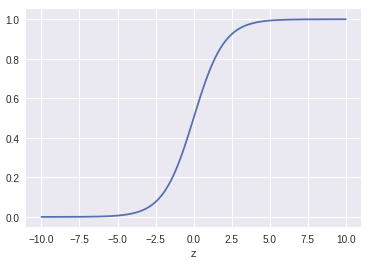
\includegraphics[width=13cm]{images/sigmoid.png}
%     \caption{シグモイド関数の形状}
%     \label{fig:シグモイド関数}
% \end{figure}



\chapter{\mc 序論}
\section{\mc 背景}
約1世紀前にHans Bergerによって世界で初のヒトの脳活動計測の試みがなされた\cite{宮内1,宮内2,宮内3}。
以降、脳活動を計測するための測定装置が開発され、
特に近年は以下の応用を目指した脳信号の解析と解読に大きな関心が寄せられている。
\begin{itemize}
    \item 医療応用:脳信号は、認知症やてんかん発作のような様々な精神障害の診断、
    および治療のために活用されている\cite{精神疾患,認知症}。
    \item 生体認証:脳信号は偽造、盗聴が困難であることから、
    固体の識別のための普遍的な生体情報となりうる\cite{個人認証,ウェアラブル個人認証}。
    \item Brain Computer Interface(BCI):
    BCIは``direct neural interface''や``brain machine interface''とも表現され、
    外界と筋肉の動作無しに相互作用するためのインターフェースの役割を担う\cite{DNI}。
    初期のBCIは麻痺患者や障害のある患者の
    生活補助装置を制御するように設計された\cite{BCIbasic}。
    更に、近年は高度な精神的タスクを実行する健常者の支援や
    仮想空間での入力装置としての商用BCIが登場するに至っている\cite{VRBCI,VRBCIsv}。
\end{itemize}
BCIにおいて脳信号を計測する方法は、大きく分けて以下の3つがある。
\begin{itemize}
    \item 侵襲式:脳へセンサを直接埋め込む方式
    \item 部分侵襲式:頭蓋骨の内部、脳の表面へセンサを埋め込む方式
    \item 非侵襲式:センサを頭蓋骨外部へ配置し、外科手術を必要としない方式
\end{itemize}
侵襲式BCIの利用範囲は安全に配慮して臨床試験に限られている。
対照的に、非侵襲式は外科手術の必要性がなく、
商業及び医療的な用途の両方に用いられており、今後更に発展する可能性があるため
本研究では非侵襲式の計測方法に着目する。

BCIで用いられる非侵襲式の計測には以下のようなものがある。
\begin{itemize}
    \item functional Magnetic Resonance Imaging (fMRI):
    MRIによって脳活動時の血流によって生ずる磁場を測定する。
    この測定は、脳の神経細胞が活動中により多くの酸素を含む血流を必要とする
    という事実に基づいている。
    \item functional Near-Infrared Spectroscopy (fNIR):
    近赤外線電磁波を用いて、
    脳皮質の異なる部分における酸素化および脱酸素化ヘモグロビンの濃度を測定する。
    \item Magnetoencephalography (MEG):
    この方法は、高感度磁力計アレイを使用して、
    脳の神経活動によって生成される磁場を直接測定する。
    MEGを利用する大きな利点は、
    頭蓋骨や他の組織は磁場に対してほとんど透明であるため、
    減衰や歪みが生じないことが挙げられる。
    \item Electroencephalography (EEG):
    この方法では頭皮上にいくつかの小さな電極を配置し、
    脳全体の神経アセンブリによって生成された電場を測定する。
    EEGは、通常、大脳皮質の表面上に位置する放射状の電流源によって
    生成される電場に敏感である。
\end{itemize}
これらの方法の中で、fMRIおよびMEGは、fNIRおよびEEGと比較して比較的高い空間分解能を提供する\cite{脳を測る}。
しかし、fMRI(図\ref{fig:fMRI})及びMEG(図\ref{fig:MEG})
は非常に高価な装置である上に大型機器であるため、
BCIアプリケーションで必要とされるような要件を満たすとは言い難い。
一方でfNIRはポータブルであるが、
脳活動から数秒程度の遅れで測定が行われるという欠点を有する\cite{脳を測る}。
\begin{figure}
    \begin{center}
    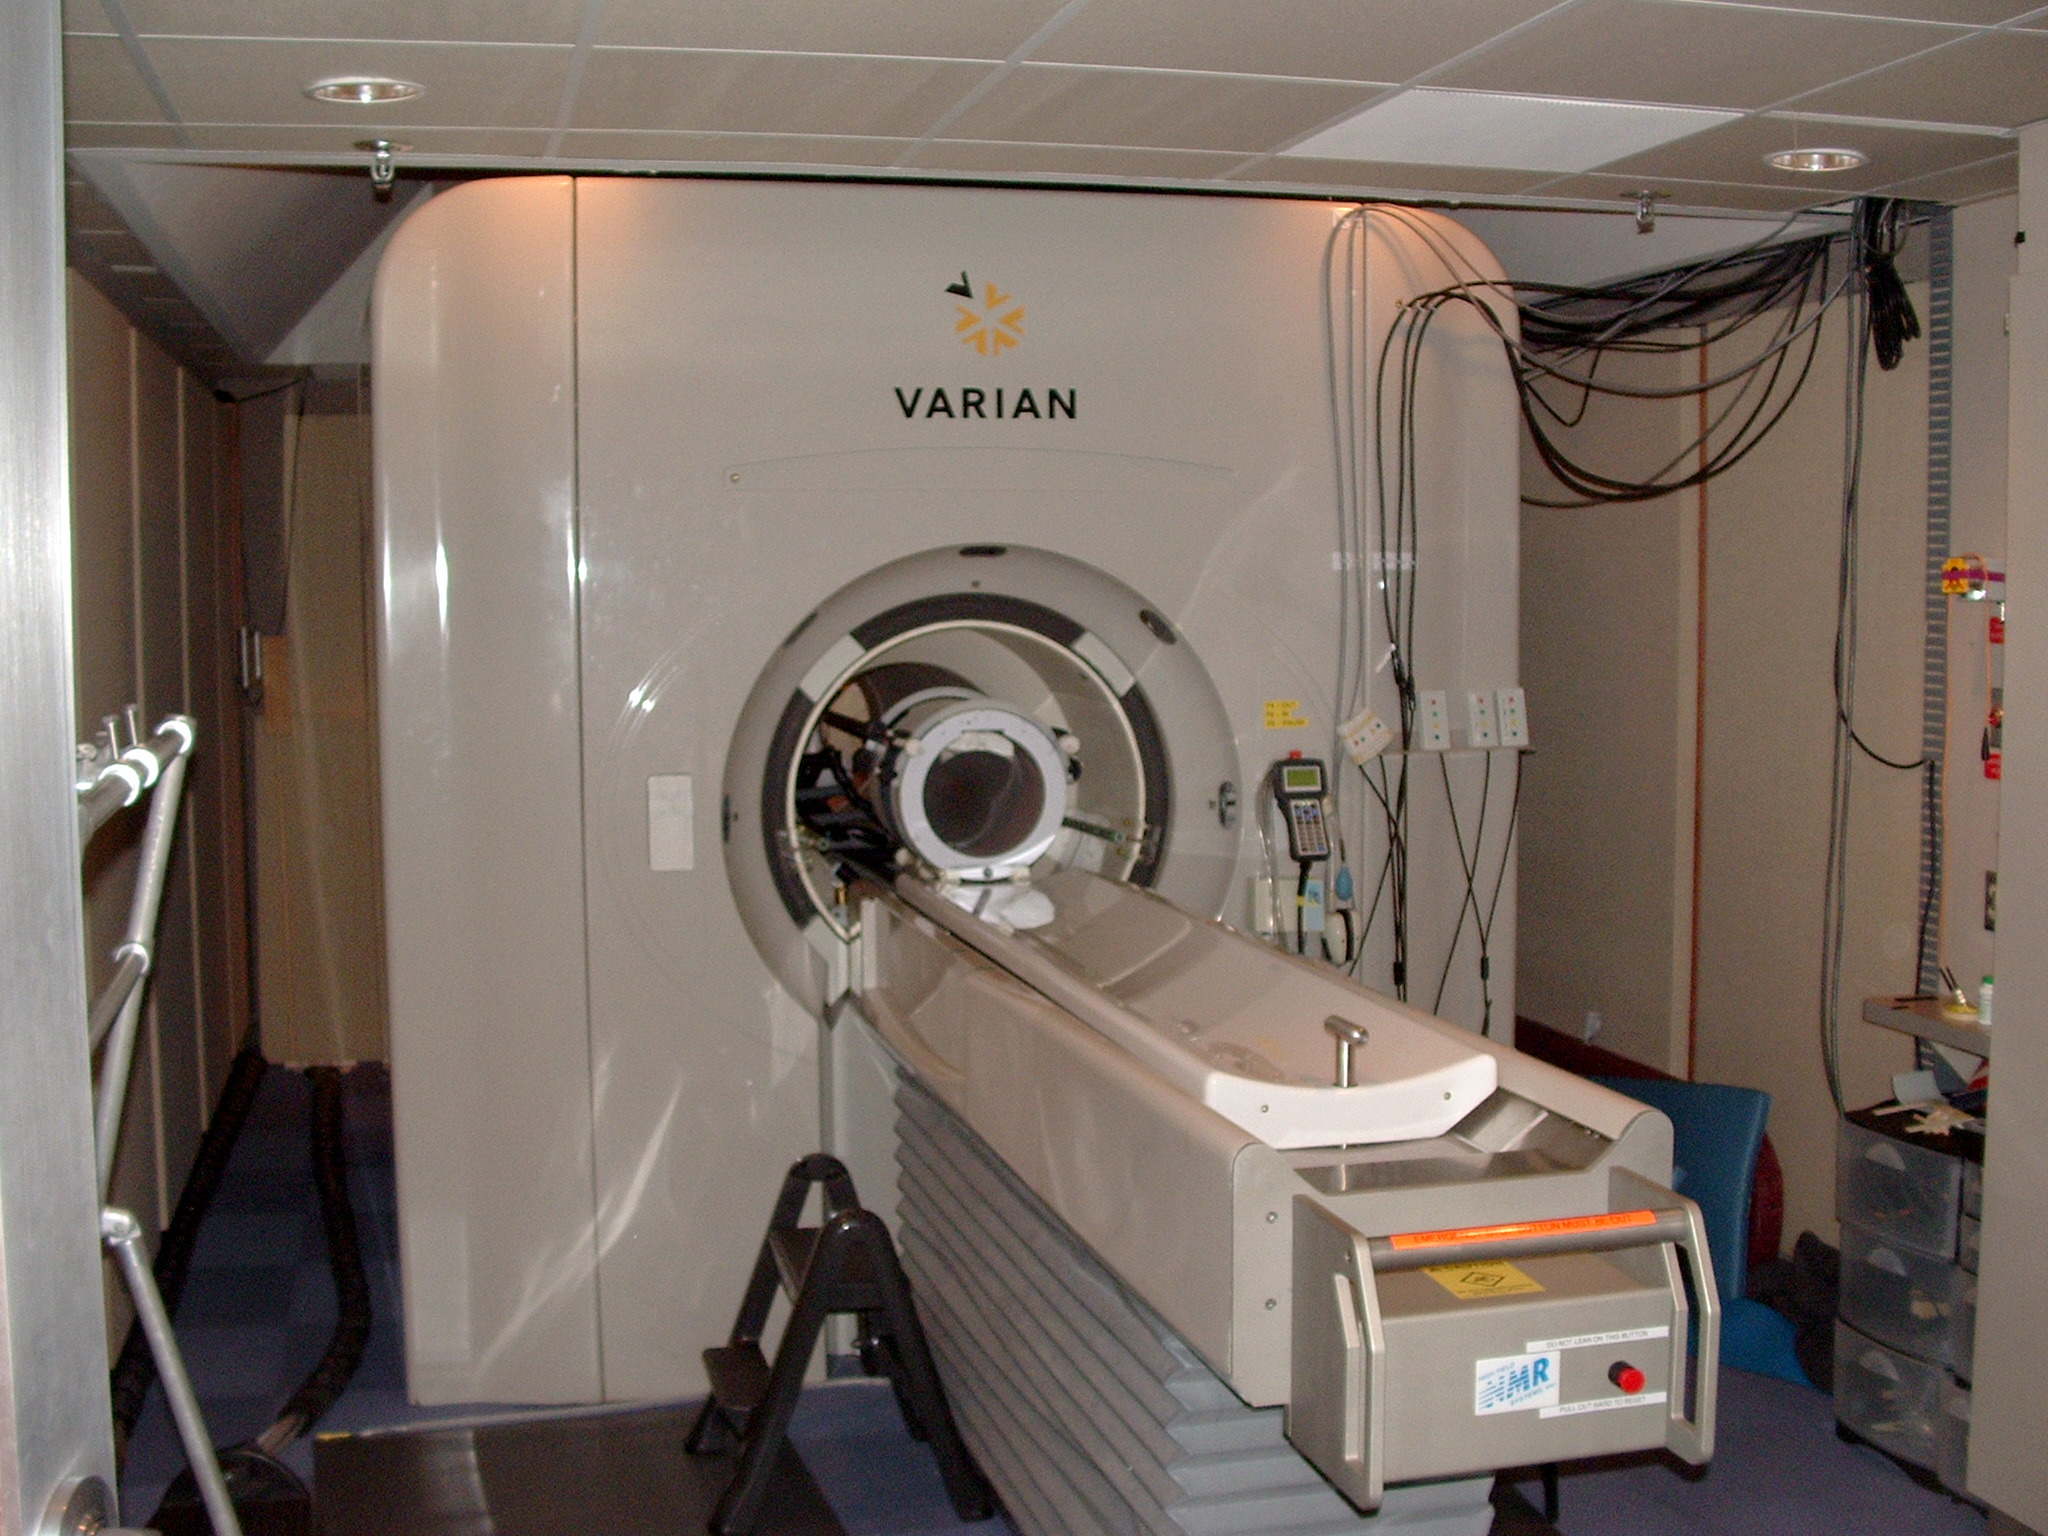
\includegraphics[width=120mm]{images/fMRI.jpg}
    \end{center}
    \caption{fMRI}
    \label{fig:fMRI}
\end{figure}
\begin{figure}
    \begin{center}
    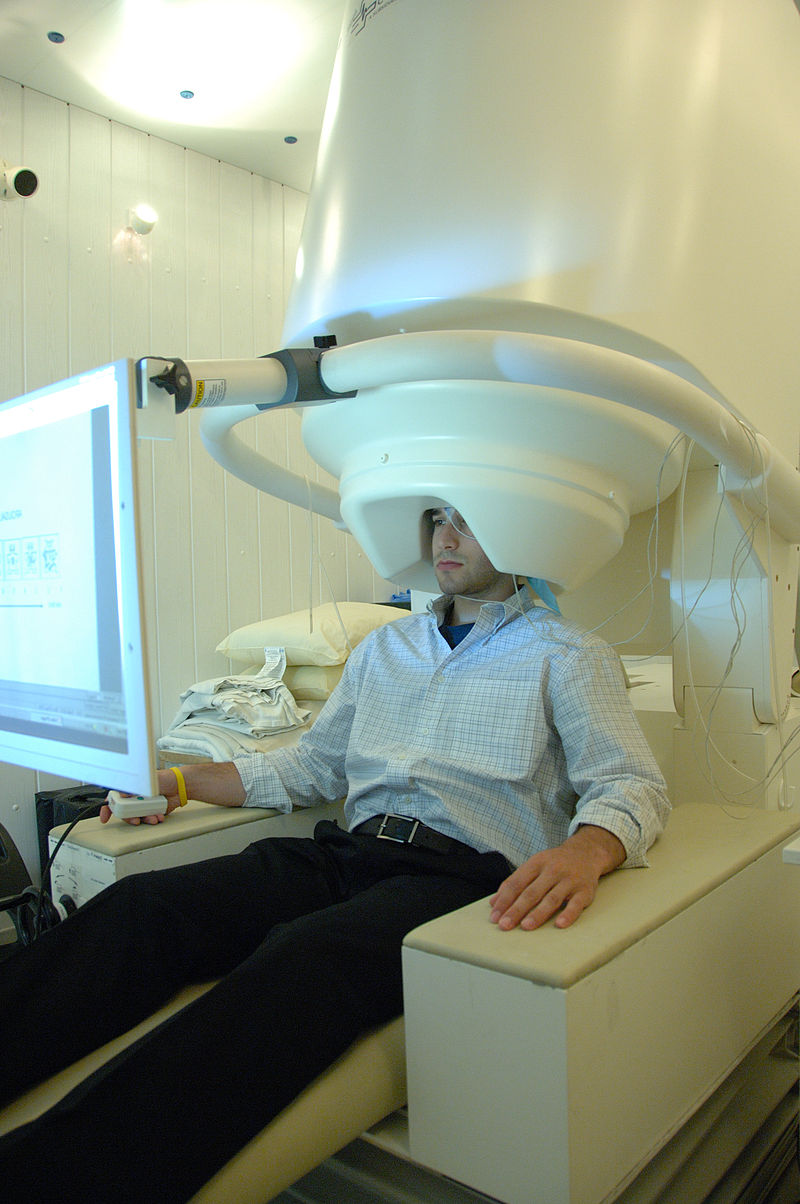
\includegraphics[width=70mm]{images/MEG.jpg}
    \end{center}
    \caption{MEG}
    \label{fig:MEG}
\end{figure}

\begin{figure}
    \begin{center}
    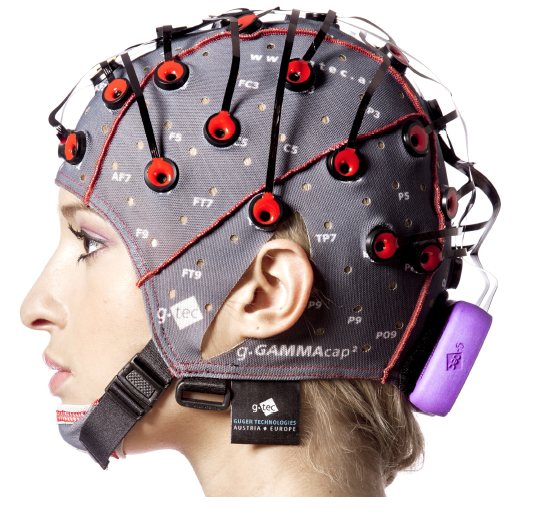
\includegraphics[width=60mm]{images/eeg.png}
    \end{center}
    \caption{EEGキャップ(ミユキ技研)}
    \label{fig:EEG}
\end{figure}
% \begin{figure}[t]
%     \begin{minipage}{0.5\hsize}
%         \begin{center}
%             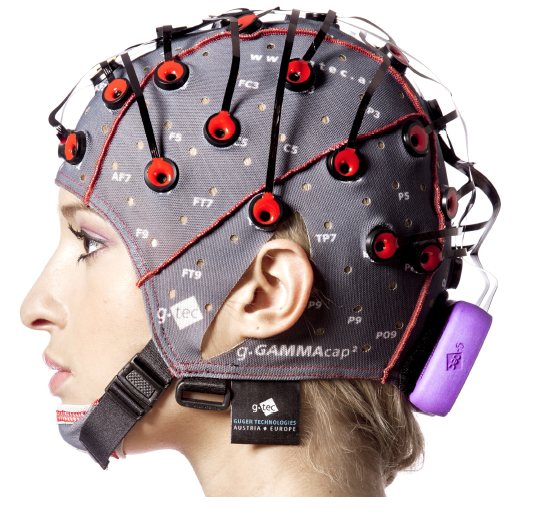
\includegraphics[width=60mm]{images/eeg.png}
%         \end{center}
%         \caption{fNIRキャップ(参照明記englishwiki)}
%         \label{fig:fNIR}
%     \end{minipage}
%     \begin{minipage}{0.5\hsize}
%         \begin{center}
%             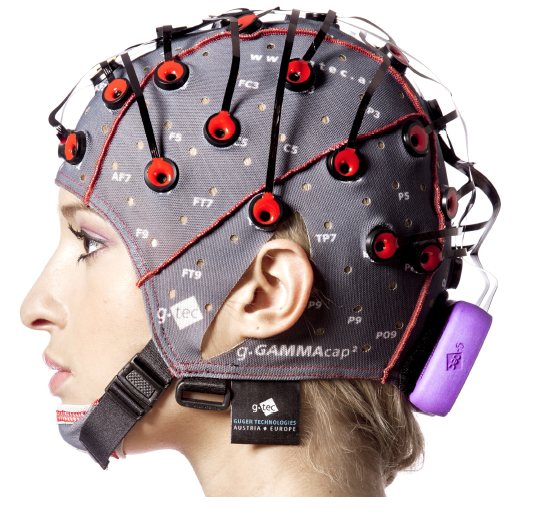
\includegraphics[width=60mm]{images/eeg.png}
%         \end{center}
%         \caption{EEGキャップ(ミユキ技研)}
%         \label{fig:EEG}
%     \end{minipage}
% \end{figure}

宮内氏の技術報告書\cite{脳を測る}によると、
EEGによる脳活動の計測に関して以下の記述がある(一部改変)。
\begin{quotation}
ヒトの脳活動計測によって獲得したいものは、精神活動・行動の生物学的基盤となる
脳の神経細胞(ニューロン)の電気的活動だが、
個々のニューロンの活動を非侵襲的に計測する事は不可能である。
しかし、ニューロンの活動に伴って様々な生理現象が生ずる。
まずニューロンが電気的な活動(一次信号)を行うためにはエネルギーを必要とし、
糖の分解のための代謝活動(二次信号)が生ずる。
酸素と糖は脳にはほとんど貯蔵されていないため、
代謝活動に伴ってエネルギーを必要としている脳の部位に関して、局所脳血流(三次信号)が増大する。
EEGやMEGは脳の電気的な活動である一次信号を計測しており、
fMRIやNIRSは血流に関する三次信号を計測している(図\ref{fig:信号フロー}\cite{脳を測る})。
\end{quotation}
\begin{figure}
    \centering
    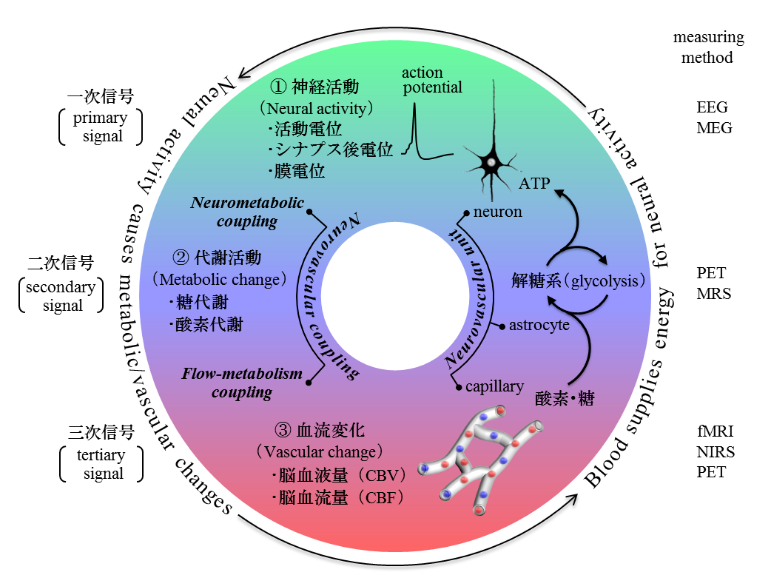
\includegraphics[width=12cm]{images/signalflow.png}
    \caption{一次信号、二次信号、三次信号と計測方法の関係図\cite{脳を測る}}
    \label{fig:信号フロー}
\end{figure}
EEGは一次信号を計測したものであり
NIRSやfMRIに比べ脳活動に対する測定値の遅れは少ないことが利点となる。
この利点に加え、EEGの測定装置は比較的安価であるため本研究の焦点とする。

続いて同様に\cite{脳を測る}にはEEGの分解能に関して以下の記述がある。
\begin{quotation}
また非侵襲計測の中では最も時間分解能が高いとされる。
ここで時間分解能とは脳の同一の場所が短時間に二回活動した場合に、
それぞれを時間的に独立した脳活動として計測できる最短の時間間隔である。
一方で頭蓋骨や皮膚、毛髪などは電位にとっては透明ではないため空間分解能は低いとされる。
ここで空間分解能とは脳の異なる部位が同時に二箇所活動した場合に、それぞれを活動部位が異なる
独立した脳活動として計測できる最小の距離である。
ただし、通常の計測においては計測装置の空間分解能や時間分解能は測定対象には依存しないが、
脳活動計測の場合においては一般的に計測対象としている現象の時空間特性や脳活動の強さ、
あるいは発生源が皮膚表面であるか脳の深部であるかなどにも依存する。
\end{quotation}
時間分解能の高さはBCIをEEGに基づいて動作させる利点となるが、
空間分解能の低さは明らかな欠点となるため、何らかの対策が必要となる。

\section{{\rm EEG}\mc に基づく{\rm BCI}{\mc の概要}}
過去20年間に、身体障害者を支援するために様々なEEGベースのBCIシステムが開発されてきた。
しかし現存するBCIシステムの大部分は、感覚刺激に応答して生成されたEEG信号である誘発電位に基づいて動作するBCIである。
\subsubsection{{\mc 誘発型}\rm BCI}
例として、ユーザがBCIシステムを使用してマウスカーソルを動作させたいとする。 
この時、異なる周波数で点滅する複数の光源をユーザに提示することで、
注視した光源に応じた誘発電位を生成させることができる。
結果として、光源を見たユーザの脳信号を分析することでマウスカーソルの動作方向を決定することが可能である。
このタイプのBCIは通常、SSVEP型BCIと呼ばれる。
他にもオドボール課題と呼ばれるタスクを課した時に生じるEEGの呼称に因んだP300型BCI
なども存在するが、外部刺激によって誘発されるタイプのBCIを本論文では誘発型BCIとまとめて表記する。
誘発電位を用いたBCIシステムは非常に正確であるが、ユーザは常に刺激に直面するため、長期的な使用には向いていない。
また、BCIシステム自体が刺激装置などの外部機器を必要とする。
\subsubsection{\mc 自発型 \rm BCI}
誘発型BCIの問題を解決するために、近年は自発的な脳活動を用いた自発型BCIの研究が盛んとなっている。
自発型BCIの中でも特に、特定の身体部位の動作を想像することで動作する運動想起型BCIに注目する。
運動想起型BCIの簡単な例を示すために、ユーザがBCIシステムを使用してマウスカーソルを動作させる例を見る。
この時、マウスカーソルを左に動かしたい場合は左手の運動を想起し、マウスカーソルを右に動かしたい場合は右手の運動を想起する。
また、下に動かしたい場合は左足、上に動かしたい場合は右足、
というように想起する身体部位に応じて外部機器への制御信号を対応させることが可能である。
同様の応用方法が車いすなどにも適用できる。
運動想起型BCIを使う利点の1つは、運動想起によって生成されたEEG信号は、
物体の想像、あるいは抽象的な概念を想像する他の精神的イメージのタスクと比較して一貫性がある点である。
一般に、運動想起によって活性化される神経は、運動を実際に実行する場合と同様であるとされる\cite{運動想起}。
本研究では運動想起型BCIに焦点を当てる。
これまでのBCIの分類について図\ref{fig:BCIclass}に示す。

\begin{figure}[tb]
    \centering
    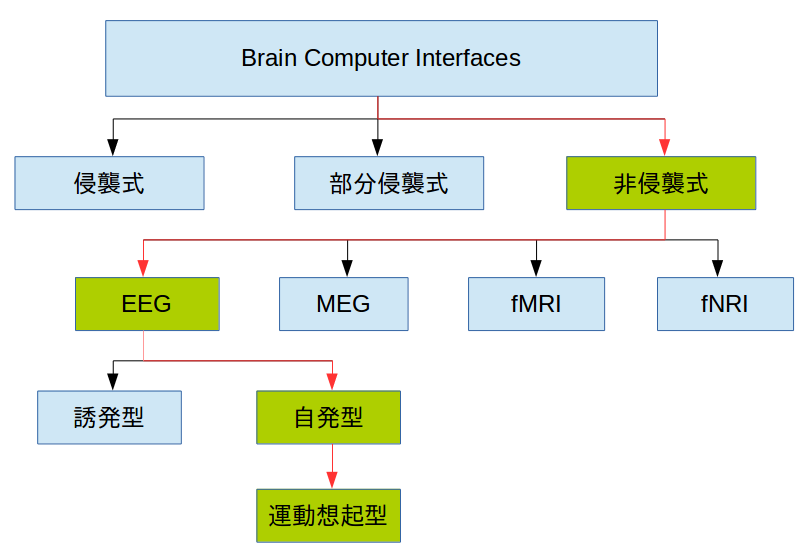
\includegraphics[width=13cm]{images/BCIclass.png}
    \caption{BCIの分類と本研究の焦点}
    \label{fig:BCIclass}
\end{figure}

\subsubsection{\rm BCI\mc の動作原理}
BCIの動作は以下のスキームに従う。
\begin{enumerate}
    \item 脳信号の獲得:センサによりアナログ信号を獲得しディジタル信号へ変換
    \item 信号の前処理:データの成形及びアーチファクトの除去
    \item 特徴量抽出:神経科学や統計に基づいた特徴量の選定
    \item 分類:特徴量から閾値に基づいて意図を分類
    \item 制御信号出力:分類結果に基づいて外部機器へ信号を出力
\end{enumerate}
BCIの種類に関わらず動作原理の根本は同様であるが、
スキームのどの段階に課題が生じるかは異なる。
侵襲式の場合は脳信号の獲得自体が非常に困難であり、安全性やメンテナンス性に課題が生ずる。
非侵襲式の場合は脳信号の獲得は気軽に実施できるが、空間分解能や時間分解能の問題、あるいは
アーチファクトの存在によって意図を復元することは容易ではない。

EEGの場合は個々の脳細胞の活動時に発生した電位の総和を頭皮上で測定しており、深さの情報は失われている。
これは侵襲式計測やMEGおよびfMRIに対する明確な欠点である。
また、頭蓋骨や人体の細胞を電位がどのように伝搬しているかは定かではないため、頭皮上の位置と
脳の表面のみを考えた場合でも位置情報は不明瞭となる。これは部分侵襲式に対する欠点となる。
従ってEEGを用いた運動想起型BCIに焦点を当てる場合、主に特徴量抽出と分類の段階が課題となる(図\ref{fig:BCIsystem})。

\begin{figure}[tb]
    \centering
    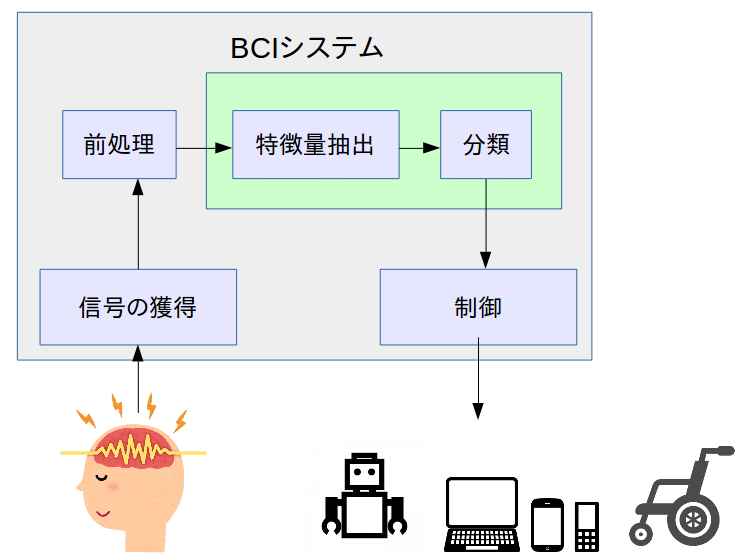
\includegraphics[width=13cm]{images/BCIsystem.png}
    \caption{BCIの動作スキーム}
    \label{fig:BCIsystem}
\end{figure}

\subsubsection{\mc 運動想起型\rm BCI\mc 周辺の研究}
運動想起時には運動野付近で特定の周波数帯域において活動電位が減少する
事象関連脱同期(Event Related Desynchronization : ERD)の存在が知られており、
神経科学的な、あるいはBCI応用のための研究が盛んに行われている\cite{ERDとERS,ERDリハビリ,運動フィードバック}。
従って特徴量としてERDが用いられる研究も数多くあり、EEGを用いた運動想起型BCIでも基礎となっている\cite{プリミティブERD,Beta波によるBCI,waveletFSVM}。
ERDを発見することができた場合、EEGの振幅あるいはパワーに閾値を設けて分類を行うことができる。
具体的にはスペクトル解析によって各周波数のパワーを推定し、パワーに閾値を設けることとなる。
しかし、EEGからのERDの検知は必ずしも容易ではない。
ERDが生じる頭皮上の位置と周波数は個人差がある上、
有効な周波数スペクトル解析に関しても未だ研究段階である\cite{時間周波数解析の比較}。

また、人の随意運動の約0.5秒から1秒前に現れる運動準備電位も特徴量になると考えられている。
実動作以前に発生するという極めて特殊な現象であるため、
その特性からBCIが人の意志に対して優れた反応速度で動作することが期待される。
BCIの研究としては実肢体動作の分類\cite{運動準備電位肢体}や実指動作の分類\cite{運動準備電位指}などがある。
実運動を行わなくとも運動準備電位が特徴量として活用できるという研究\cite{運動準備電位想起,運動準備電位想起2}もある。

一方で特定のEEGの現象を直接獲得せずに運動想起型BCIを構築する手法も提案されており、
それらの多くが統計的信号処理や機械学習を活用したものである。
特にCommon Spatial Pattern(CSP)と呼ばれる統計的信号処理\cite{CSP1990,CSP1999}は、
EEG解析のために発案されて以降、現在までに様々な派生手法を生み出している\cite{csssp,正則化CSP,カーネルCSP,cvscsp}。
その中でもFilter Bank Common Spartial Pattern\cite{fbcsp}と呼ばれるCSPの
発展手法は、ERDに基づくBCIも含め他の手法と比べ高い性能を有している。

現在、EEGの現象として知られている既知の特徴量を検知する手法から、
機械学習や統計的信号処理を活用した特徴量抽出手法と高度な分類器を組み合わせ
高い性能を発揮する手法の模索が行われている\cite{BCIの比較}。

\section{\mc 目的}
\subsection{\mc モチベーション}
BCIを構築するためにEEGの解析を行うことで性能の向上を達成しようとする試みも続いている\cite{脳波解析BCI,脳波分析BCI,ERSBCI}。
EEGではBCIに限らず、頭皮領域と周波数帯域に関しての研究が盛んに行われてきたため、
特徴量抽出を行う場合にも電極と周波数に着目する場合が多い。
特にERDは特定の周波数における電位の減少であるため、
スペクトル解析と時間周波数解析が有効利用でき、
現在も運動想起型BCIのための研究が行われている\cite{時間周波数解析の比較}。
これらの研究は基礎科学として重要な役割を担うが
BCIを実際に応用する場面を考慮すると、
BCI構築前に大量のEEGを計測しなければならないなど
個々人のEEGの解析が必須である手法には限界がある。

また、綿密なEEGの解析を実施するか否かに関わらず、
左手を動作させる場合と右手を動作させる場合とでは脳の活動は事実異なっている。
タスク間でのEEGの違いを可視化したい場合や、
脳機能自体を解明したい場合には綿密なEEGの解析は有効であるが
、その際には解析はあくまで人間が解釈する手段であり、
解析のために処理された信号がそのままBCIを用いる際の特徴量として有望だとは限らない。
% 本論文では、BCIが動作するための特徴量抽出を
% 人間が解釈できる形で与える必要はないと主張する。
なぜなら人間がデータを解釈、あるいは可視化できるような形に加工することで
分類に有用な情報が失われている可能性もあるためである。

更に統計的信号処理や機械学習に基づく
特徴量抽出手法と分類手法にも数多くの種類が存在する。代表的なものを以下に記す。
この中の幾つかは第\ref{chapter:BCIのための要素技術}章にて解説する。
\begin{itemize}
    \item Laplacian Filter(LF)
    \item Principal Component Analysis(PCA)
    \item Independent Component Analysis(ICA)
    \item Canonical Correspondence Analysis(CCA)
    \item Common Spartial Pattern(CSP)
    \item バンドパスフィルタバンク
    \item フーリエ変換
    \item ウェーブレット変換
    \item 自己回帰モデル
    \item Emperical Mode Decomposition(EMD)
    \item Linear Discriminat Analysis(LDA)
    \item Support Vector Machine(SVM)
    \item Logistic Regression(LR)
\end{itemize}
これらの手法はBCIの構成要素として組み込まれるが
数多くある手法の中から個々人に応じて、
あるいはタスクに応じて適切に組み合わせるのは容易ではない。


\subsection{\mc 達成目標}
個人事に綿密なEEGの解析を行う必要性が残る限り、
専門家が常にいる医療の現場などの特定の分野でのみしかBCIの発展は望めない。
またBCIを構成するための考えうる手法の組み合わせは無数にあり、
決定的なアーキテクチャが存在しないと言える。
そこでまずは、個人事のEEGの解析を行うこと無く入力から出力までのBCIの構成を
データから一貫して推定する``End to End学習''の手法を提案する。

End to End学習を達成するために、
音声認識と画像認識の分野で既に大きな成功を収めている
ニューラルネットワークに着目した。
BCIとして考えうる構成と、ニューラルネットワークを用いたBCIの構成図を図\ref{fig:BCIpattern}に示す。
\begin{figure}
    \centering
    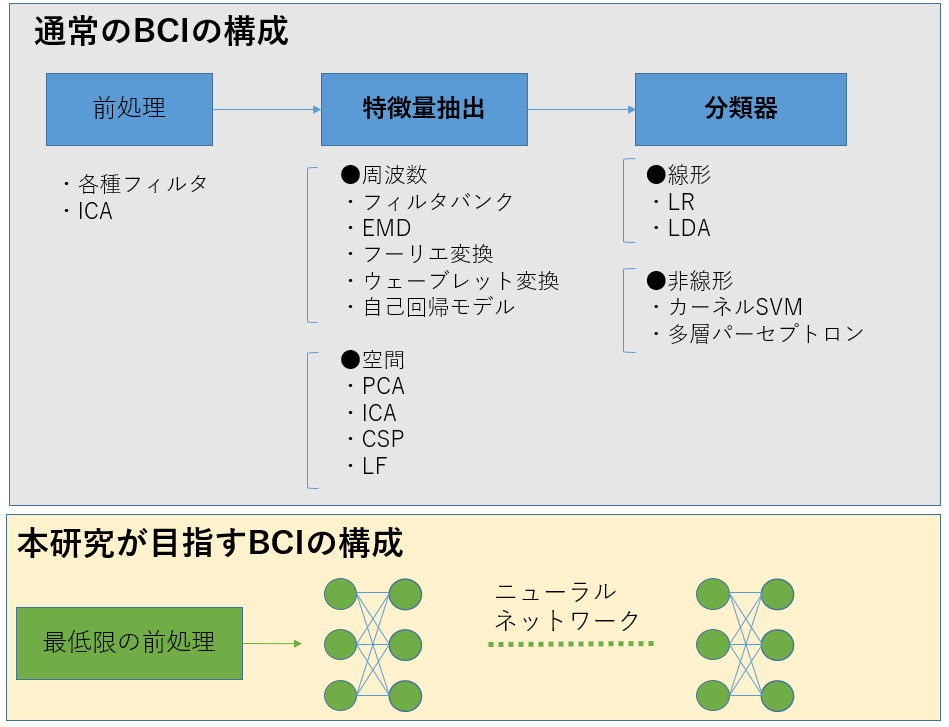
\includegraphics[width=12cm]{images/BCIpattern.PNG}
    \caption{従来のBCIの構成と本研究が目指すBCIの構成}
    \label{fig:BCIpattern}
\end{figure}
またEnd to End学習を提案することによって以下の項目について達成することを目標とした。
\begin{itemize}
    % \item タスク毎のEEGの解析の必要性を排除
    \item 各個人におけるEEGの解析の必要性を排除
    \item 人類に共通した一般的なBCIの可能性を示す
\end{itemize}

``各個人におけるEEGの解析の必要性を排除''はEnd to End学習の直接的な貢献であるが、
更に``人類に共通した一般的なBCIの可能性を示す''ことで基本的なBCIの大枠を獲得しておき、
個々人に応じて比較的少量のデータからキャリブレーションを行う
転移学習の可能性を示唆することができる\cite{転移学習}。


% また、ニューラルネットワークの応用研究が盛んな画像認識の分野では、
% 既に模範的なニューラルネットワークの構造が発見されており、
% 大量の画像によって事前学習を行い、
% 達成したい認識対象を絞り込んだ後に転移学習することで
% 手軽に高い性能の分類器が得られる。
% 従って、BCIにおいて模範的なニューラルネットワークの構築により
% 以下の事項が達成できる可能性が示唆される。
% 従って研究の成果によって以下の項目において貢献することができる。

% また、マルチモーダルなBCIの一部としても応用可能である。

% 更に、モデルの構築も含めハイパーパラメータの存在によって
% 試行錯誤の必要性も非常に高い。
% しかし、特徴量抽出手法や分類器自体を変更しながら様々な組み合わせを検討することに比べ、
% ニューラルネットワークの調整は単純作業である。
% また今後ハイパーパラメータの調整自体を自動化する、
% あるいは学習に組み込む方法も出現する可能性がある。




\chapter{{\rm BCI}{\mc のための要素技術}}
\label{chapter:BCIのための要素技術}
この章ではBCIに用いられる要素技術について述べる。
ここで紹介する技術はBCIに限らずデータを扱う場面で広く持ちいられている手法であるため、
一般的な定式化と用途を述べた後に、脳波解析における応用方法や問題点について述べる。

\section{\mc 周波数解析}
スカラーの時間波形\(x(t)\)に対して、周波数スペクトルを算出する際に用いられるフーリエ変換について述べる。
\(t\)が連続量である時\(x(t)\)をアナログ信号と呼び、離散的であればディジタル信号と呼ぶ。
このセクションではアナログ信号とディジタル信号が混在するため、
アナログ信号に関しては\(x(t)\)と表記し、ディジタル信号を\(x_n\)と表記することで明確に区別する。
\subsection{4\mc 種類のフーリエ変換}
時間を連続的に扱うか離散的に扱うかの違いだけでなく、
周波数を連続的に扱うか否かによってもフーリエ変換の式は異なっており、\(2\times 2 = 4\)つのフーリエ変換がある。
通常はフーリエ変換について議論する場合は時間も周波数も連続であるとみなした式を使う場合が多いが、
コンピュータ上で数値の処理を行う場合は原則離散的であるため、4つのフーリエ変換について全て簡単に説明する。

\subsubsection{\mc フーリエ変換}
スカラーの時間波形\(x(t)\)に対して、フーリエ変換は以下の(\ref{eq:FT})で表され、
逆フーリエ変換の式は(\ref{eq:iFT})で表される。
\begin{equation}
    X(\Omega)=\int_{-\infty}^{\infty} x(t)\exp(-i\Omega t)dt
    \label{eq:FT}
\end{equation}
\begin{equation}
    x(t)=\frac{1}{2\pi} \int_{-\infty}^{\infty} X(\Omega)\exp(i\Omega t)d\Omega
    \label{eq:iFT}
\end{equation}
ここで、\(i\)は虚数単位であり\(X(\Omega\))は\(\Omega\)を変数とするスカラー関数である。
逆フーリエ変換はスカラーの時間波形\(x(t)\)をある周波数\(\Omega\)の波形\(\exp(i\Omega t)\)の
線型結合によって表現した式である。このときの結合係数が\(X(\Omega)\)である。
工学的な立場では時間波形\(x(t)\)が与えられた時に、波形\(\exp(i\Omega t)\)による線型結合をすることで、
波形にどのような周波数の波形がどれくらいの割合で含まれているかを知りたいケースがある。
それを可能にするのがフーリエ変換であり、\(x(t)\)から結合係数\(X(\Omega)\)を算出することが可能である。
通常はこの時の結合係数\(X(\Omega)\)を周波数スペクトルと呼ぶ。
逆フーリエ変換(\ref{eq:iFT})に登場する定数倍\(1/2\pi\)は、フーリエ変換\(\cal F(\cdot)\)と逆フーリエ変換\({\cal F}^{-1}(\cdot)\)が、
フーリエ変換可能な時間波形\(x(t)\)に対して
\({\cal F}^{-1}({\cal F}(x(t))) = x(t)\)となるように調整するための係数である。
この係数は逆フーリエ変換の式ではなくフーリエ変換の式に付いていてもよく、あるいは両方の式に平方根の形で分配されていても構わない。
またフーリエ変換可能な時間波形とは以下を満たす\(x(t)\)である
\begin{equation}
    \int_{-\infty}^{\infty}|x(t)|dt < \infty
\end{equation}

\subsubsection{\mc 離散周波数フーリエ変換}
取りうる周波数を離散的にした場合のフーリエ変換について説明する。
離散周波数フーリエ変換という命名は便宜的にこの論文内で行っているものであり一般的ではない。
通常、ここで紹介するフーリエ変換は「フーリエ級数展開」として知られている。
歴史的には微分方程式を解くために開発され、フーリエ変換よりも先に発見されている。
離散周波数フーリエ変換と離散周波数逆フーリエ変換はそれぞれ(\ref{eq:sFT})と(\ref{eq:siFT})で表される。
\begin{equation}
    X_k=\frac{1}{T_0}\int_{-\frac{T_0}{2}}^{\frac{T_0}{2}} x(t)\exp(-i\Omega_0 kt)dt
    \label{eq:sFT}
\end{equation}
\begin{equation}
    x(t)=\sum_{k=-\infty}^{\infty} X_k \exp(i\Omega_0 k t)
    \label{eq:siFT}
\end{equation}
離散周波数逆フーリエ変換は、スカラーの時間波形\(x(t)\)を離散的な周波数\(\Omega_0 k\)の波形\(\exp(i\Omega_0 k t)\)の
線型結合によって表現した式である。このときの結合係数が\(X_k\)である。
ここに\(T_0\)は時間波形の周期であり、\(\Omega_0 = 2\pi/T_0\)を基本周波数と呼ぶ。
離散周波数フーリエ変換が、時間波形が与えられた時の周波数スペクトルを算出する役割を担うことは、フーリエ変換と同様である。
フーリエ変換との最たる違いは、時間波形に対して周期性を仮定している点であり、その周期は既知でなければならない。
時間波形が周期性を持つ場合には周波数は離散的な値を取る。

\subsubsection{\mc 離散時間フーリエ変換}
取りうる時間を離散的にした場合のフーリエ変換について説明する。
離散時間フーリエ変換と離散時間逆フーリエ変換はそれぞれ(\ref{eq:tFT})と(\ref{eq:tiFT})で表される。
\begin{equation}
    X(\omega)=\sum_{n = -\infty}^{\infty} x_n \exp(-i\omega n)
    \label{eq:tFT}
\end{equation}
\begin{equation}
    x_n=\frac{1}{2\pi} \int_{-\pi}^{\pi} X(\omega) \exp(i\omega n)d\omega
    \label{eq:tiFT}
\end{equation}
離散時間逆フーリエ変換が、時間波形\(x_n\)を周波数スペクトル\(X(\omega)\)を結合係数とした
\(\exp(i\omega n)\)の線型結合を表しているのはこれまでと同様である。
しかし、離散時間フーリエ変換では周波数スペクトル\(X(\omega)\)が周期的な関数となることは
強調しておかねばならない。

\subsubsection{\mc 離散フーリエ変換}
離散フーリエ変換は、取りうる時間も周波数も離散的であるとした場合のフーリエ変換である。
離散フーリエ変換と離散逆フーリエ変換はそれぞれ(\ref{eq:tsFT})と(\ref{eq:tsiFT})で表される。
\begin{equation}
    X_k=\sum_{n = 0}^{N-1} x_n \exp \left(-i\frac{2\pi}{N} k n \right)
    \label{eq:tsFT}
\end{equation}
\begin{equation}
    x_n=\frac{1}{N}\sum_{k=0}^{N-1} X_k \exp \left(i \frac{2\pi}{N} k n \right)
    \label{eq:tsiFT}
\end{equation}
ここで\(N\)はサンプル時間点数の意味で周期である。
時間波形に対する周期は\(N\)であるが、周波数スペクトルに対する周期も\(N\)となる。
仮に1周期が1000点のサンプル点によって構成される時間波形に対し離散フーリエ変換を用いた場合は、
得られる周波数スペクトルは1000点で周期を有する形式となる。
離散フーリエ変換は有限の数列から有限の数列への変換であり、他のフーリエ変換と異なり無限大を扱う必要はないため
コンピュータ上で計算を実行することが可能である。
高速フーリエ変換と呼ばれる実応用で頻繁に用いられるアルゴリズムは、
離散フーリエ変換(\ref{eq:tsFT})を高速に実行する手続きのことである。

\subsection{\mc パワースペクトル密度}
パワースペクトル密度\(PSD(\Omega)\)とは時間信号\(x(t)\)の周波数スペクトルを\(X(\Omega)\)とした時、
\begin{equation}
    PSD(\Omega)=|X(\Omega)|^2
    \label{period}
\end{equation}
に相当する関数である。
信号\(x(t)\)のエネルギーが周波数\(\Omega\)に関してどのように分布するかを示している。
コンピュータでパワースペクトル密度を計算する場合は(\ref{eq:tsFT})で計算される\(X_k\)
の二乗\(|X_k|^2\)を算出する。
しかし、数学的な定式化を行う上では以下の定義が用いられ、\(|X_k|^2\)はピリオドグラムと呼び区別する。
\begin{equation}
    PSD(\Omega) = \int_{-\infty}^{\infty} R(\tau)\exp(-i\Omega \tau)d\tau
    \label{eq:wh_theorem}
\end{equation}
ここに、\(R(\tau)\)は
\begin{equation}
    R(\tau)  =  \mathbb E[x(t)x(t+\tau)]    
\end{equation}
であり、信号\(x(t)\)の自己相関関数である。(\ref{eq:wh_theorem})は、ウィーナー・ヒンチンの定理としても知られており、
自己相関関数のフーリエ変換がパワースペクトル密度になることを示している。
この定義から明らかなようにパワースペクトル密度とは統計量であって、
解析的に算出されるのではなく、推定されるものである。

ピリオドグラムはパワースペクトル密度の推定を行う手段として用いられる。
一般的にピリオドグラムによる推定値は平均と標準偏差が同じ大きさを持ち、
時系列の長さを長くしても推定誤差は改善されない。
時系列を長くすることで周波数分解能を高くすることはできるが、
個々の周波数でのスペクトルの相対誤差は変化しない。
そこで、通常は何らかの平滑化を行って個々の周波数成分の推定値の誤差を減少させる方法が一般に採用される。
主な方法として、時間領域で波形を分割し、複数のピリオドグラムの平均を算出する方法がある。
時間領域で波形を分割する際には、波形が時間で互いに重なりを持つように分割する、Welchのオーバーラッピング法が用いられる。
また最大エントロピー法を用いてパワースペクトル密度を推定する方法もあり、
その場合には(\ref{eq:wh_theorem})を制約条件としたエントロピー最大化の変分問題を解くこととなる。
このパワースペクトル密度推定方法はバーグ法として知られている。
スペクトル解析に関する記述は書籍\cite{スペクトル解析}に詳しい。

脳波は、運動想起時に特定の周波数領域でエネルギーが減少する事象関連脱同期が生じるとされているため、
適切な電極選定を行い、
脳波のパワースペクトル密度\(PSD(\Omega)\)を推定することができれば、
とある\(\Omega\)で著しくパワーが減少する様子が確認できる。
\section{\mc 多変量解析}
多変量解析とは多変量データを統計的に扱う手法である。
扱うデータの科学的知識に基づいた特徴量抽出に加え、実データの統計的な性質を考慮した
特徴量抽出も様々な分野で行われている。
この章では脳波解析で用いられている多変量解析について紹介し、
その有用性と限界について考察する。

\subsection{\rm Principal Component Analysis(PCA)}
Principal Component Analysis(PCA)は特徴量抽出手法として幅広い分野で活用されている。
簡単のため時間平均が\(0\)の多次元信号\(x(t)\in \mathbb R^D\)に対してPCAによる特徴抽出を考える。
PCAでは変換行列\(W^T \in \mathbb R^{D \times D}\)を左から作用させ、特徴量
\begin{equation}
    z(t)=W^Tx(t) \in \mathbb R^D
\end{equation}
を獲得するが、この際、\(z(t)\)の各成分が互いに無相関になるように\(W\)を決定する。
\(z(t)\)が無相関となるためには、その分散共分散行列\(\Sigma_z=\mathbb E[z(t)z^T(t)]\)が対角行列になることが要請される。
ここで\(x(t)\)の分散共分散行列を\(\Sigma_x=\mathbb E[x(t)x^T(t)]\)とすると、\(z(t)\)の分散共分散行列\(\Sigma_z\)について
\begin{eqnarray}
    \Sigma_z & = & \mathbb E[z(t)z^T(t)] \nonumber \\
    & = & \mathbb E[W^Tx(t)x^T(t)W] \nonumber \\
    & = & W^T \mathbb E[x(t)x^T(t)]W \nonumber \\
    & = & W^T \Sigma_x W
    \label{eq:var}
\end{eqnarray}
と表すことができる。(\ref{eq:var})が対角行列になるような\(W\)は、\(\Sigma_x\)の固有値分解によって求まる。
今、\(\Sigma_x\)のD個の固有値を\(\lambda_1 \geq \cdots \geq \lambda_D\)とする。
この固有値を対角成分に並べた行列を\(\Lambda={\rm diag}(\lambda_1,\cdots,\lambda_D )\)とすると、
\(\Sigma_x\)の固有値分解は、ある\(U\)が存在して以下の形式となる。
\begin{equation}
    \Sigma_x=U \Lambda U^{-1}
\end{equation}
\(U^{-1}\)を左から、\(U\)を右から掛けることで\(U^{-1}\Sigma_x U=\Lambda\)が得られ、
\(U^{-1}=W^T\)で\(U=W\)とすれば(\ref{eq:var})への要請を直ちに満たす。
これは\(W^T=W^{-1}\)という条件が満たされれば良く、
実数信号の分散共分散行列\(\Sigma_x\)は一般に正定値実対称行列となっており、
直交行列によって固有値分解が可能であるため条件を満たす。
また、このとき全ての\(i\)について固有値\(\lambda_i\)は正の値となり、
固有値\(\lambda_i\)に属する固有ベクトルにデータを射影した際の分散を表す。
これらの数学的な扱いやすさからPCAは非常に広く普及している。

\begin{figure}[t]
    \begin{minipage}{0.5\hsize}
     \begin{center}
      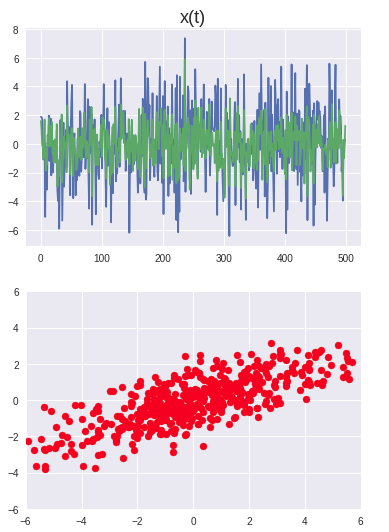
\includegraphics[width=70mm]{images/x(t).png}
     \end{center}
     \caption{x(t)の波形と散布図}
     \label{fig:x(t)}
    \end{minipage}
    \begin{minipage}{0.5\hsize}
     \begin{center}
      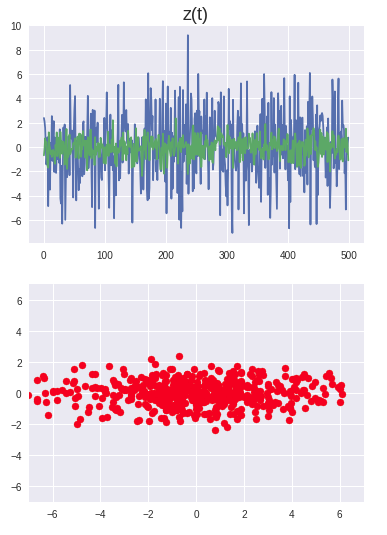
\includegraphics[width=70mm]{images/z(t).png}
     \end{center}
     \caption{z(t)の波形と散布図}
     \label{fig:z(t)}
    \end{minipage}
\end{figure}
\begin{figure}
    \centering
    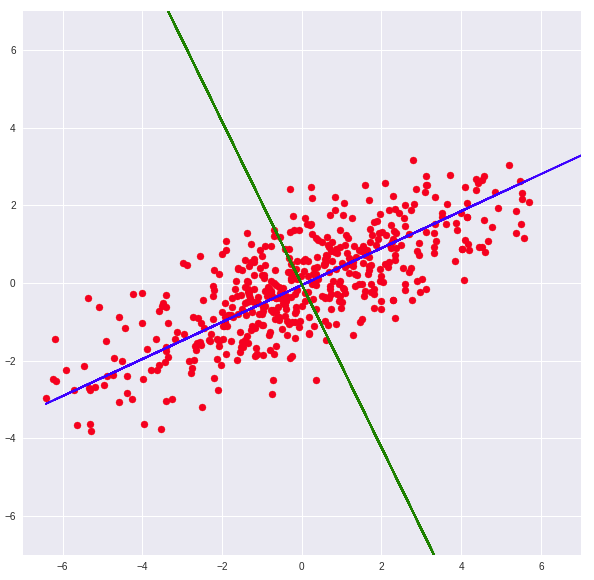
\includegraphics[width=12cm]{images/z=Wx.png}
    \caption{PCAによって得られる基底}
    \label{fig:z=Wx}
\end{figure}

PCAの働きを見るため\(D=2\)とした場合の線形変換\(z(t)=W^Tx(t)\)を図で確認する。図\ref{fig:x(t)}は人工的に作成した2次元波形\(x(t)\)と各成分の散布図である。
この\(x(t)\)に対してPCAを用いると、
図\ref{fig:z(t)}に示す\(z(t)\)が得られ、散布図から
\(z(t)\)の各成分は無相関となっていることが確認できる。
図\ref{fig:z=Wx}は\(x(t)\)に対してPCAを施した場合に得られる新たな直交基底を表しており、
\(z(t)\)は新たな直交基底に\(x(t)\)を射影したものに他ならない。
PCAでは基底を取り直すことで各成分が無相関な信号を獲得でき、
その結果、新たに得られた信号の各成分がどのような意味を持つのかを考察しやすくなる。

しかし、応用上は単に基底を取り直すことを目的とするケースは少ない。
通常は固有値分解によって求まった固有ベクトル(新たな基底)を全て利用するのではなく、
値の大きな固有値に属する固有ベクトル\(w\)を\(d(<D)\)個選び、
\(W_{d} = (w_1, \cdots, w_d)\)によって変換行列を構成することで、
\begin{equation}
    z(t)=W_{d}^Tx(t) \in \mathbb R^d
    \label{reduction}
\end{equation}
と次元削減を行う。
値の大きな固有値に属する固有ベクトルによって基底を構成することは、
\(W_d\)による基底の元で、信号の分散(あるいは振幅)が最大化されることを要請することと等価である。
また、射影先での分散最大化に伴い、(\ref{reduction})での変換行列\(W_d\)は、
元々の信号\(x(t)\)と、\(x(t)\)を\(\mathbb R^D\)の部分空間
\(\mathbb R^d\)へ射影した信号\(z(t)\)との二乗誤差を最小化する変換行列となっている。


以上からPCAは、元々の信号\(x(t)\)の情報損失を二乗誤差の意味で最小限に抑えながら、
射影先で大きな変動を有し、かつ各成分が無相関となる特徴量\(z(t)\)を抽出する。しかし、脳波への応用を考える上ではPCAの性質は必ずしも有効には働かない。
運動想起BCIを考える上では、脳波に含まれる全ての情報の中から識別したい身体部位に関する情報のみを抽出する必要がある。
この場合、脳波信号のごく一部のみが重要である可能性があり、射影先で大きな分散を持つような信号となっているかは定かではないためである。




\subsection{\rm Indipendent Component Analysis(ICA)}
Indipendent Component Analysis(ICA)はPCAを発展させた比較的新しい信号解析手法である。
ICAはPCAと同様に変換行列\(W^T \in \mathbb R^{D \times D}\)を左から作用させ、特徴量
\begin{equation}
    z(t)=W^Tx(t) \in \mathbb R^D
\end{equation}
を獲得するが、この際、\(z(t)\)の各成分が互いに独立になるように\(W\)を決定する。
独立性は無相関性の十分条件であり、PCAに比べて\(z(t)\)により強い条件を要請する。
PCAでは無相関性が固有値分解という数学的によく知られた問題と関連していたが、独立性は簡単な問題への定式化は困難であるため、
通常は独立性を測る目的関数を設定し、勾配法などの逐次最適化法を用いる。
ICAの求解アルゴリズムを述べるのは本研究テーマから逸脱するため、主要なアルゴリズムに絞って簡単に説明する。
最も普及している求解アルゴリズムはFastICAとして知られており、
独立性の必要条件である無相関性を要請した後、独立性を最大化することで解を得る。
無相関性を満たすようにするためには前処理としてPCAを用いることができる(正確にはPCAを用いた中心化と白色化処理が行われる)。
前処理後は独立性の最大化問題が、\(z(t)\)の各成分のエントロピー最小化問題に変換されるが、
この最小化問題も容易ではない。従って更にネゲントロピーなる量を導入し、最大化問題に書き換える。
ネゲントロピーは信号の非ガウス性を測る尺度であり、ガウス分布から遠いほど大きな値となる。
FastICAではネゲントロピーの最大化を各成分ごとに順次取り出していく。
この時、非ガウス性が高い成分の順番に取り出されていく。独立成分分析の解説は次の文献が詳しい\cite{ICA1}\cite{ICA2}。

図\ref{fig:ica_pca}にPCAとICAの振る舞いをトイデータを用いて比較を掲載する。
図\ref{fig:ica_pca}のbase vectors of ICA and PCAから分かるようにICAで得られる基底は直交するとは限らない。
また、PCAの基底の大きさは等しく\(1\)であり正規直交基底を構築するが、ICAでは正規性も持つとは限らない。
\begin{figure}
    \centering
    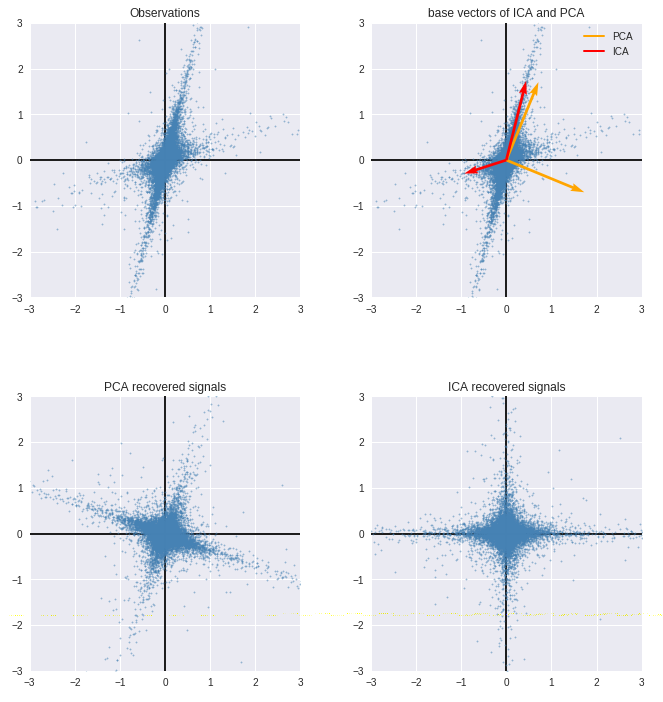
\includegraphics[width=15cm]{images/ica_pca.png}
    \caption{無相関な基底を得るPCAと独立な基底を獲るICAの比較}
    \label{fig:ica_pca}
\end{figure}


脳波への応用では、脳波計測時に混入した脳波以外の信号(筋電位、眼電位など)が脳波とは統計的に独立であると考え、
脳波以外の信号成分を除去する目的で利用される。一方で運動想起BCIにおいて身体部位に関する脳波成分を直接抽出することはPCA同様に難しい。
筋電などの場合、脳波と独立であるという仮定は妥当であり、
かつ振幅が目視可能なほど脳波に比べて大きくなる。従って、ICAによって分解された独立な成分から筋電などを見分けるのは比較的容易である。
しかし、一方で身体部位に関する脳波成分がその他のあらゆる脳波と独立であるかは定かではなく、仮に独立であった場合にも分解された信号から
目視によって特定することは困難であると推察される。

\subsection{\rm Blind Source Separation(BSS)}
上記ではPCAとICAが次元削減として用いられることを見た。
一方でこれらの手法はBlind Source Separation(BSS)問題の解法として解釈されることも多いため、
ここで簡単に述べておく。
まず信号源\(s(t)\ \in \mathbb R^d\)を直接観測できない場合に、
\(D\)個のセンサで\(x(t) \in \mathbb R^D\)という信号を観測したとする。
このとき、観測信号\(x(t)\)のみから信号源\(s(t)\)を推定する問題がBSS問題である。
計測機器や環境に応じて、信号源\(s(t)\)は何らかの変換\(f(\cdot)\)を受けて観測されると考えられる。
従って\(x(t)\)は
\begin{equation}
    x(t)=f(s(t))
\end{equation}
と表記できる。このときに観測に伴う変換\(f(\cdot)\)が線形変換\(A\)であると仮定した場合、
\begin{equation}
    x(t)=As(t)
    \label{eq:bss1}
\end{equation}
と表記することができ、BSS問題は\(x(t)\)から\(A\)と\(s(t)\)を同時に推定する問題であると見なせる。
ここで仮に適当な線形変換によって、観測信号\(x(t)\)を
\begin{equation}
    z(t)=Wx(t)
    \label{eq:bss2}
\end{equation}
と変換することを考える。
\(W\)を上手く選ぶことに成功すれば、\(z(t)=Wx(t) \simeq s(t)\)となることが期待できる。
ここで\(D=d\)、すなわち信号源の次元と観測信号の次元が一致している場合を考える。
このとき(\ref{eq:bss1})において、
\(A\)が正則であるとし、
\begin{equation}
    s(t)=A^{-1}x(t)
\end{equation}
と表すことが可能になる。従って、(\ref{eq:bss2})の\(W\)を\(W=A^{-1}\)とすることができれば、
\begin{equation}
    z(t)=Wx(t)=A^{-1}x(t)=s(t)
\end{equation}
と信号源を求めることが可能である。
ただし、\(z(t)=s(t)\)となる\(W\)が存在するとしても、
既知の\(x(t)\)に対して未知の\(W,s(t)\)を求めようとしている状況に変わりはなく、BSS問題は基本的に不良設定問題である。
また、実データでは信号源と観測信号の次元が一致しない場合が多く\(A\)は逆行列を持たないため、
状況はより複雑である場合が多い。通常はBSS問題を解くためには何らかの条件を追加するか、
正則化の手法を導入する必要がある。
PCAやICAは信号源\(s(t)\)が各成分について無相関あるいは独立であると仮定することで条件式を追加し、
観測信号\(x(t)\)から条件式を満たすような\(W\)と\(z(t)\)を求め、
\(z(t)\)が信号源\(s(t)\)の良い近似になっていると考えるBSS問題の解法の一種である。

PCAとICAのBSS問題への振る舞いを確認するために、トイデータによる実験結果を図\ref{fig:bss}に示す。
周波数の異なる2つの正弦波と1つのノコギリ波にそれぞれガウスノイズを加算した信号源(図\ref{fig:bss}のTrue Sources)
を準備し、適当な線形変換を施して観測信号(図\ref{fig:bss}のObservations)とする。
図\ref{fig:bss}のICA recoverd signalsがFastICAによって推定された信号源に適当なゲインを加えたものであり、
図\ref{fig:bss}のPCA recoverd signalsがPCAによって推定された信号源に適当なゲインを加えたものである。
ICAでは周波数の異なる正弦波とノコギリ波を明確に分解できており、
信号源に近い波形が得られていることが確認できるが、
PCAでは信号源と異なる信号が得られている。
PCAの振る舞いは各成分を無相関にしつつ、射影先で分散を最大化するような基底を求めるため
ノコギリ波と位相が一致している正弦波を1つの成分に集約してしまっている。

\begin{figure}
    \centering
    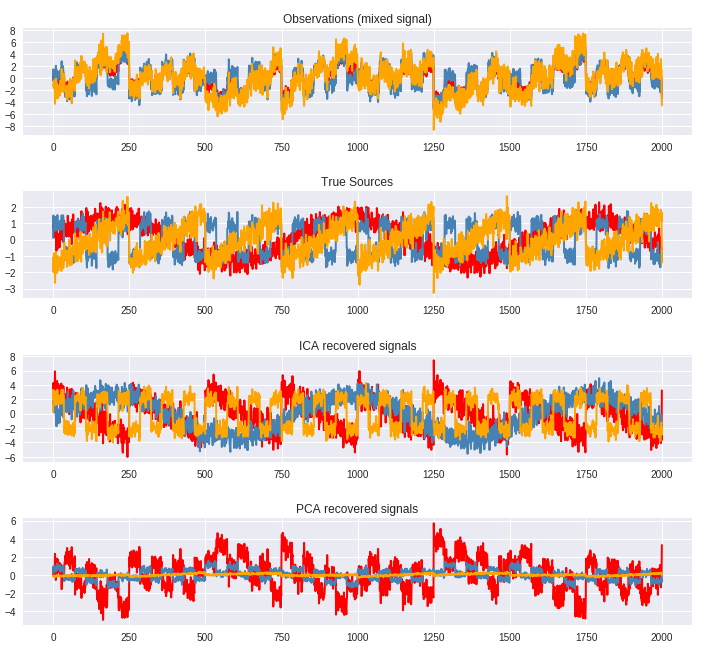
\includegraphics[width=15cm]{images/bss.png}
    \caption{BSS問題に対するPCAとICA}
    \label{fig:bss}
\end{figure}

トイデータによる実験ではICAがBSS問題に対して有効に働くことが確認できるが、
本来信号源がどのようなものであるかは未知であるため、
信号源推定が正しく行われたかを確認するのは実データでは困難である。
運動想起BCIを想定して脳波にBSS問題を適用する場合には、観測された信号\(x(t)\)
から脳波信号の根源である\(s(t)\)を復元することを目的とするが、ICAによって推定された信号源の
いずれの成分が運動想起と関連しているのかを判別するのは極めて難しい。
ただし、脳波と筋電では波形が明らかに異なるため、筋電と脳波が独立であるという仮定を用いて
ICAによって筋電成分を取り出すことは可能である。
一般に、不良設定問題であるBSS問題に対しては何らかの仮定を置かざるを得なく、
複雑な脳波に対して適切な仮定を設けることが重要な課題となる。
\section{分類手法}
分類問題の説明を行う。

\subsection{Linear Discriminant Analysis(LDA)}
\label{subsec:LDA}
Linear Discriminant Analysis(LDA)は統計分析において伝統的に用いられてきた歴史ある手法である。
特にBCIではCSPによる特徴量抽出の後に用いられることが多い。
LDAでは多次元データを部分区間で切り取り、部分空間で分類超平面を構築することでクラス分類を行う。
分類超平面を構築する手段を与えなければ、LDAは特徴量抽出手法としても機能する。
まず、多次元データ\(x\in \mathbb R^D\)を基底\(w \in \mathbb R^D\)へ射影すると、
以下の式で表されるスカラー値を獲得できる。
\begin{equation}
    z = w^Tx \in \mathbb R
\end{equation}
zに対してある閾値を設定し、\(z \geq -w_0\)の場合はクラス\(C_1\)とし、そうでない場合は
クラス\(C_2\)であるとすることで分類器を獲得できる。
多次元データを1次元空間へ射影した場合には多くの情報損失が生ずるが、
\(w\)の取り方を上手く調整することによって、クラス分離を行いやすい射影を選択できる。
クラス分類性能を向上させる\(w\)を得るために、まず以下のようにクラス毎の平均ベクトル\(m_1,m_2\)を定義する。
\begin{eqnarray}
    m_{1} & = & \frac{1}{|C_1|}\sum_{x\in C_1}x  \\
    m_{2} & = & \frac{1}{|C_2|}\sum_{x\in C_2}x
\end{eqnarray}
ここに、\(|C_i|\)はクラス\(C_i\)に属するデータの数である。
クラス\(C_1\)とクラス\(C_2\)の平均が射影先で大きな値となれば分離が行われやすいと想定できる。
従って、以下の距離の最大化によって分類性能が向上すると考えられる。
\begin{equation}
    d=|w^T(m_1-m_2)|
    \label{eq:dis}
\end{equation}
しかし実際にはクラス毎の平均を考慮しただけでは分類が上手く行くとは限らない(図\ref{fig:mean_dis})。
射影先での各クラスのデータの分散が大きい場合には、異なるクラスのデータが重なってしまう場合が生じるからである。
\begin{figure}
    \centering
    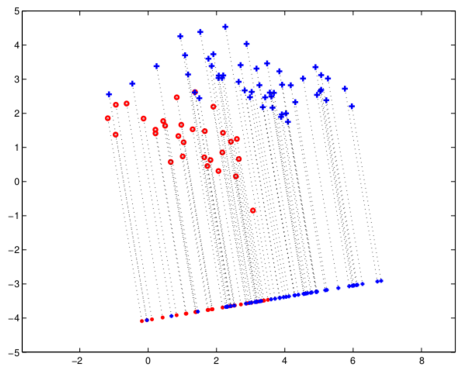
\includegraphics[width=12cm]{images/mean_dis.png}
    \caption{クラス毎の平均間の距離を射影先で最大化した判別分析}
    \label{fig:mean_dis}
\end{figure}
この問題を解決するためにはデータの分散を考慮する必要がある。
まず射影先での各クラスの分散は以下で表記できる。
\begin{eqnarray}
    \sigma^2_{1} & = & \sum_{x\in C_1}\{w^T(x-m_1)\}^2  \\
    \sigma^2_{2} & = & \sum_{x\in C_2}\{w^T(x-m_2)\}^2
\end{eqnarray}
ここで、全データのクラス毎の分散の和を総クラス内分散として以下で定義する。
\begin{equation}
    \sigma^2  = \sigma^2_1 + \sigma^2_2
    \label{eq:sig}
\end{equation}
総クラス内分散(\ref{eq:sig})を小さくしながらクラス間の平均の距離(\ref{eq:dis})を大きくすることを考慮し
LDAでは以下の評価関数を用いる。
\begin{eqnarray}
    J(w) & = & \frac{d^2}{\sigma^2} \nonumber \\
    & = & \frac{\{w^T(m_1-m_2)\}^2}{\sum_{x\in C_1}\{w^T(x-m_1)\}^2 + \sum_{x\in C_2}\{w^T(x-m_2)\}^2}
\end{eqnarray}
このクラス間の平均とクラス内の分散を考慮した評価関数を用いることで、
射影先でデータがクラス毎に小さくまとまり、かつ異なるクラスのデータがなるべく離れるようになる(図\ref{fig:var_dis})。
\begin{figure}
    \centering
    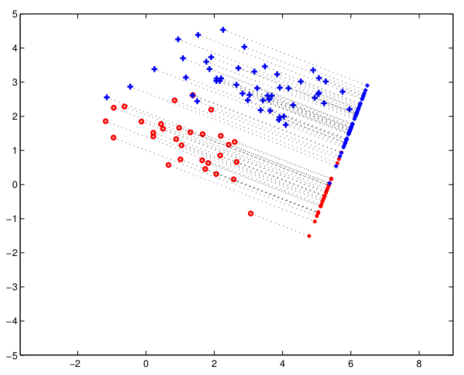
\includegraphics[width=12cm]{images/var_dis.png}
    \caption{クラス毎の平均間の距離を射影先で最大化した判別分析}
    \label{fig:var_dis}
\end{figure}

1次元の空間(数直線上)でクラス毎にデータが上手く分離できた後、
数直線上に閾値\(w_0=(m_1+m_2)/2\)を設けることで分離平面が得られる。
これはクラス毎の平均値の平均値によって分離平面を設定したことに相当する。
しかし、射影のされ方によってはこの閾値は適当ではない。
より精密な分類を行うためには、\(z=w^Tx\)がクラス毎に異なるガウス分布から生じる確率変数だと考え、
クラス\(C_i\)の条件付き確率\(p(z|C_i)\)を算出した判別基準を設け、条件付き確率が大きいクラスへ分類するなどの方法を取る。
% ガウス分布を仮定した場合における判別基準は、マハラノビス距離が近いクラスへ分類することと等価である。
% 必ずしもガウス分布であるという仮定は必要ないが、\(z\)は複数の確率変数の線型結合であるため
% 中心極限定理によりこの仮定は正当化されうる。


\subsection{Support Vector Machine(SVM)}
脳波の分類ではSupport Vector Machine(SVM)の応用例もある。
基本的にSVMはマージン最大化の考えによって汎化性能の向上に成功した
2クラス分類のための線形分類器である。まずマージン最大化という概念について説明する。
マージンとは端的に述べるとデータ点と分類超平面との距離のことを表す。
学習データに対してマージンを最大化することで、学習データが空間上で僅かに移動した際にも
誤分類を起こしづらくなると期待できる。
SVMではこのマージン最大化によって以下の分類超平面を定める。
\begin{equation}
    y(x) = w^Tx + w_0
    \label{eq:displane}
\end{equation}
ここに\(x\)は\(D\)次元のデータベクトルであり、\(w\)は\(D\)次元のパラメータベクトルである。
\(w_0\)もスカラーパラメータであり閾値の役割を担う。
分類面の役割により\(y(x)\)は\(x\)がクラス\(C_1\)に属する場合には正の値を、\(C_2\)に属する場合には負の値を取るように学習される。
ここで、(\ref{eq:displane})の超平面と、あるデータ点\(x_n\)との距離は以下で表される。
\begin{equation}
    |r| = \frac{|y(x_n)|}{|w|}
    \label{eq:distance}
\end{equation}
ここで、\(x_n\)がクラス\(C_1\)に属する場合は\(t_n=1\)とし、クラス\(C_2\)に属する場合には
\(t_n=-1\)と定めた\(t_n\)を導入する。
さらに\(x_n\)には分類面から最も近いデータ点のみを考慮することとし、
そのときの\(|r|\)をマージンと呼び以下で表す。
\begin{equation}
    |r|_{margin} = \min_{x_n}\frac{t_ny(x_n)}{|w|}
    \label{eq:margin}
\end{equation}
この(\ref{eq:margin})を最大化するようにパラメータを決定することで
マージン最大化を実現することができる。
従って、SVMのパラメータ決定は以下の最適化問題によって定式化される。
\begin{equation}
    \argmax_{w_0,w}\left(\min_{x_n}\frac{t_ny(x_n)}{|w|}\right)
    \label{eq:obj margin}
\end{equation}
しかしこの最適化問題において、\(w,w_0\)の大きさは本質的ではない。
なぜなら\(w,w_0\)を同時に\(kw,kw_0\)と定数倍した場合にも(\ref{eq:margin})の値は変化しないためである。
従って、\(w,w_0\)の大きさに関して制約を設ける必要がある。
そこで分類面から最も近い\(x_n\)に関して\(t_n(w^Tx+w_0)=1\)
となるような制約を\(w,w_0\)に対して要請する。
この条件式に伴って、任意のデータ点において\(t_n(w^Tx+w_0) \geq 1 \)という制約が与えられる。
最終的にマージン最大化問題(\ref{eq:obj margin})は以下で定式化される。
\begin{equation}
    \begin{aligned}
    & \argmin_{w_0,w}
    & & \frac{|w|^2}{2}  \\
    & \text{s.t.}
    & &  t_n(w^Tx+w_0)  \geq 1 
    \end{aligned}
    \label{eq:obj nonlinear}
\end{equation}
目的関数の分母は、単に勾配を計算する際に約分できるというテクニックによるものである。
分子の二乗は、最適化問題の解を変更せずに勾配計算などを容易に行うための変形である。
図\ref{fig:margin}に分類面の定め方によりマージンが異なっている様子を見ることができる。
左右いずれの図も学習データに対して正しく分類が行える分類面になっているが、
新規のデータに対しての分類結果が異なってくる。SVMでは右図の分類面の方が優れていると考える場合に用いる手法である。
\begin{figure}
    \centering
    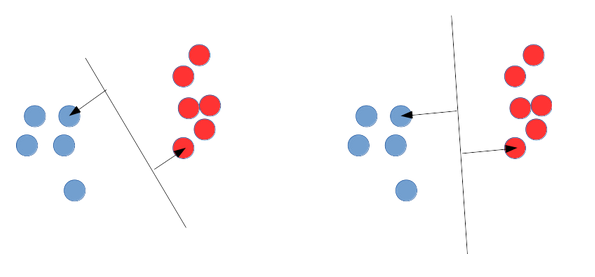
\includegraphics[width=12cm]{images/margin.png}
    \caption{分類面によってマージンの大きさが異なる様子}
    \label{fig:margin}
\end{figure}
ここまで線形分類を行う場合のSVMを見てきたが、
一般的に線形分類器はデータ点を非線形関数\(\phi(\cdot)\)によって別の特徴空間へ写像し、
特徴空間上で線形分類を行う問題へ拡張することができる。SVMでは分類超平面を以下の式によって構築することに相当する。
\begin{equation}
    y(x) = w^T \phi (x) + w_0
    \label{eq:displane}
\end{equation}
この場合においてもこれまでと同様の議論で最適化問題を以下のように定式化できる。
\begin{equation}
    \begin{aligned}
    & \argmin_{w_0,w}
    & & \frac{|w|^2}{2} \\
    & \text{s.t.}
    & &  t_n(w^T\phi(x)+w_0)  \geq 1 
    \end{aligned}
    \label{eq:obj nonlinear}
\end{equation}

実データは線形分離不可能な場合が多いため、
通常SVMを用いる場合は上記のような非線形に拡張されたものを用いる。
また実データは異なるクラスのデータが重なって分布することも多々あるため、
厳密な分類を行うことは不可能な場合が多い。
そういった場合に対応したソフトマージンと呼ばれる考えがあり、
学習データの誤分類に対して寛容になる指標を導入する。
このソフトマージンの考え方は機械学習で過学習抑制に用いられる正則化の考えと本質的には変わりない。
また、制約付き最適化問題をラグランジュ法によって変形することで双対問題を獲得することができる。
双対問題においては非線形変換後の空間での内積のみが必要となり、
具体的な非線形変換の計算をデータ\(x\)に対して実施する必要はない。
すなわち、非線形変換\(\phi(x)\)による特徴空間への写像を具体的に考える代わりに、
最終的に計算の必要性がある内積\(\phi(x)^T\phi(x')\)を定義することでSVMの非線形への拡張が可能である。
このような方法はカーネル法として知られており、このときに用いられる内積計算をカーネル
\(k(x,x')=\phi(x)^T\phi(x')\)と呼ぶ。カーネルを定めることが特徴空間の設計を行うことに相当するが、
BCIも含めた多くの応用では既に知られた優れた性質を持つカーネルを活用することがほとんどである。
以下に代表的なカーネルについて記載する。
\begin{description}
    \item[・線形カーネル:非線形変換を行わないことに対応。] \mbox{}
    \begin{center} \(k(x,x')=x^Tx'\) \end{center}
    \item[・多項式カーネル:多項式関数による非線形変換に対応。] \mbox{} 
    \begin{center} \(k(x,x')=(x^Tx' + c)^M\) \end{center}
    \item[・ガウス基底カーネル:特徴空間が無限次元となる。] \mbox{}\par
    \begin{center} \(k(x,x')=\exp\left(-\frac{|x-x'|^2}{2\sigma^2}\right)\) \end{center}
\end{description}
通常、カーネルを用いる場合にはハイパーパラメータが付随する。多項式カーネルの場合は\(c,M\)、
ガウス基底カーネルの場合は\(\sigma\)がハイパーパラメータとなり、これらの調整次第で
得られる分類面は異なる。
 
応用上はソフトマージンカーネルSVMを用いればよく、ソフトマージンのハイパーパラメータとカーネルの設計を変えることで
通常の線形SVMの働きをさせることも可能である。
ソフトマージンカーネルSVMの識別関数は以下で表される。
\begin{equation}
    y(x) = \sum_{n=1}^Na_nt_nk(x,x_n) + b
    \label{dis_kernel}
\end{equation}
ここで学習データの数を\(N\)としている。
また最適化問題は以下で定式化される。
\begin{equation}
    \begin{aligned}
    & \argmax_{a_1,\cdots,a_N}
    & & \sum_{n=1}^N a_n - \frac{1}{2}\sum_{i=1}^N \sum_{j=1}^N a_ia_jt_it_jk(x_i,x_j) \\
    & \text{s.t.}
    & & 0 \leq a_n \leq C  \\
    & & &  \sum_{n=1}^N a_nt_n=0
    \end{aligned}
    \label{eq:kernel SVM}
\end{equation}
ここに\(C\)はソフトマージンのハイパーパラメータであり、誤分類に対しての厳しさを表す。
最適化問題の解である\(a_1,\cdots,a_N\)と任意の\(n\)を選んで以下の条件式に代入することで閾値\(b\)も求まる。

\begin{equation}
    t_n\left( \sum_{m=1}^Na_mt_mk(x_n,x_m) + b \right)=1
    \label{eq:bias}
\end{equation}
ただし、(\ref{eq:bias})は無駄な計算も含まれている。\(a_n=0\)となるような\(x_n\)に対して
\(\sum_{n=1}^Na_nt_nk(x,x_n)\)の計算を実行する必要はない。
\(a_n\neq0\)となっている\(x_n\)のことをサポートベクトルと呼び、
実際にはサポートベクトルのみ計算に考慮すれば良い。
このことは新規のデータに対して(\ref{dis_kernel})の計算を行うときも同様である。
従って学習後に保持しておかねければならないデータはサポートベクトルのみに限定でき、
実用上省メモリに貢献できる。

\subsection{Logistic Regression(LR)}


\chapter{{\mc 従来の運動想起型}{\rm BCI}}
この章ではまず、BCIのために開発された解析手法であるCommon Spatial Patternについて紹介する。
その後、前章の要素技術を含めた従来の運動想起型BCIの構成方法について述べ、課題点を明らかにする。

%%%%%%%%%%%%%% 特徴量工学の説明 %%%%%%%%%%%%
\section{特徴量工学}
図\ref{fig:EEGfootmove}と図\ref{fig:EEGhandmove}はそれぞれ足の運動想起と手の運動想起を行った際の脳波である。
いずれも0秒以前は以前はディスプレイを注視した状態であり、0秒以降に運動想起を4秒間行っている。
電極の個数は64個用いられており、全ての電極の波形が表示されている。
足の運動想起が行われているのか手の運動想起が行われているのかを脳波の生データから識別するのは困難であることが分かる。
運動想起BCIの標準的な役割は、脳波信号\(x(t)\in \mathbb R^D\)に対応した運動想起部位を識別することであるが、
そのためには脳波の生データに対して何らかの処理を施し、識別に有用な特徴を見出さねばならない。
ここに\(D\)を電極の個数である。
\begin{figure}[t]
    \centering
    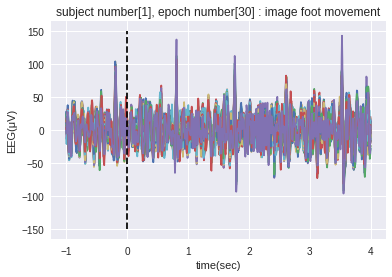
\includegraphics[width=9cm]{images/EEGfootmove.png}
    \caption{0秒〜4秒間に足の運動想起を行った際の脳波(EEG)}
    \label{fig:EEGfootmove}
\end{figure}
\begin{figure}[t]
    \centering
    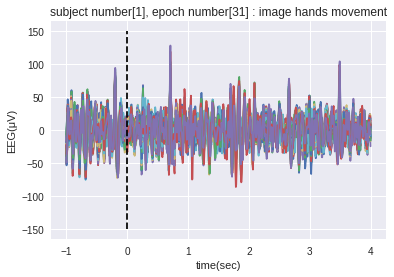
\includegraphics[width=9cm]{images/EEGhandmove.png}
    \caption{0秒〜4秒間に手の運動想起を行った際の脳波(EEG)}
    \label{fig:EEGhandmove}
\end{figure}
そこで、何らかの変換\(f(\cdot)\)を脳波信号\(x(t)\)に対して施すことで、
特徴量\(z=f(x(t))\)の獲得を目指すのが特徴量工学である。

\subsection{他分野での特徴量工学}
特徴量工学はBCIに限らず、データ解析を必要とする多くの分野で活用されている。
例えば画像処理の分野では、画像に写っている物体の輪郭を
抽出するエッジ処理や、画像に対してぼかしを入れる平滑化処理などが特徴量抽出手法として用いられる。
また音声認識の分野では、音声の周波数に重要な情報が含まれていると考え、
周波数スペクトルやケプストラムなどを特徴量として用いる試みがなされてきた。

\subsection{脳波解析における特徴量工学}
特に脳波







% \section{その他の手法}
% \subsection{スペクトログラムを特徴量とする手法}
% 運動想起型BCIでは、上記までに述べてきたCSPによる手法が非常に活発に議論されている。
% しかし、CSPによる手法は計測の際に多数の電極を用いる必要がある。
% 一方で実用上は電極が少なければ少ない程計測における負担は少なくなるため、
% 少数の電極のみを用いてBCIを構築する方法も研究がされている。
% 例として運動時、あるいは運動想起時には特定の頭皮領域に配置された電極において、
% 特定の周波数帯域にパワーの減少が生じること(事象関連脱同期)が知られているため、
% この現象に狙いを定めてBCIを構築する研究も盛んである。

% この手の手法の主な流れを示す。まず脳波信号を\(X \in \mathbb{R}^{M \times N}\)と表記する。ここに、\(M\)は電極の個数、\(N\)は計測時間点数である。
% 電極に対しての重み付け係数(空間フィルタ)$w \in \mathbb{R}^M$を何らかの方法で決定することで、
% \begin{equation*}
%     z = w^T X \in \mathbb{R}^N    
% \end{equation*}
% と変換する。次に$z$に対して短時間フーリエ変換${\cal F}(\cdot)$を行い、
% \begin{equation*}
%     A = {\cal F}(z) \in \mathbb{R}^{F\times N}
% \end{equation*}
% を獲得する。短時間フーリエ変換の代わりにウェーブレット変換などの時間周波数解析を用いる場合もある。
% スペクトログラム$A$から事象関連脱同期を見出すことができれば、ある特定の周波数帯域でのパワーを見張ることで運動の意図推定が可能となる。
% 実際、特定の周波数帯域のパワーに対して閾値を設けることで、運動意図推定を行う手法も提案されている。
% ただし、事象関連脱同期が生じる周波数帯域には個人差があることが想定されるため、スペクトログラム$A$に対して何らかの行列分解を用いて特徴量を取り出すことも提案されている。



% \subsection{Convolutional Neural Networks(ConvNets)}
% この手法に関しては\cite{deepconv}を参照されたい。



\section{Common Spatial Patternとその派生手法}
運動想起型BCIに対しては``Common Spatial Pattern(CSP)''\cite{csp}が1999年に提案されて以降、
非常に活発に応用研究がされている。その後、ベンチマークとして引用されてきただけでなく、
CSPの拡張手法も数多く提案されてきた。
CSPは脳波解析の分野で発展した手法であるため、その定式化も脳波計測時のデータ構造に合わせた
形式となっている。そのため、今一度脳波信号の定式化を述べた後にCSPについて記す。

\subsection{脳波信号の定式化}
これまで多次元の信号を\(x(t)\in \mathbb R^D\)と表記し、連続時間信号として扱ってきた。
しかし、通常は計測された脳波はコンピュータで処理するために
離散時間信号\(x_n \in \mathbb R^D\)に変換される。
従って、以降、脳波信号を離散時間信号として取り扱う。
また、運動想起時の脳波信号を計測する際には、
被験者に対して定められたタイムスケジュールで運動想起を行うように指示がなされる。
例として64個の電極を用い、サンプリング周波数100Hzで10秒間の計測を行った場合、
計測された運動想起1回分の脳波信号は\(X \in \mathbb{R}^{64 \times 1000}\)
と表すことができる。従って、以降統一のため、\(M\)を電極の個数、
\(N\)を計測時間点数とした場合の脳波信号を以下で定義する\begin{equation}
    X =(x_1, \cdots, x_N)\in \mathbb{R}^{M \times N}\    
\end{equation}


運動想起を\(K\)回行った場合には、\(K\)個の\(X\)が得られる。
通常は運動想起時の脳波を数個から数十個集め、統計的な指標を元に有用な特徴量を抽出する。
CSPは運動想起BCIに対して極めて有効に働くとされている特徴量抽出手法である。


\subsection{Common Spatial Pattern(CSP)}
\label{subsec:CSP}

CSPを脳波に用いる際は、脳波信号\(X\)を直接扱うのではなく、何らかの前処理を施した信号\(\hat{X} = {\cal H}(X) \)を用いる。
通常、\(\cal H\)には、運動想起に関連のある周波数帯域のみを通過させるバンドパスフィルタを用いる。
バンドパスフィルタ通過後の脳波信号を以下のように表記する。
\begin{equation}
    \hat X = \left( \hat x_1,\cdots,\hat x_N \right) \in \mathbb{R}^{M \times N}
\end{equation}
\(\hat x_i \in \mathbb R^M\)における添字\(i\)はサンプル時刻の添え字である。
CSPでは、新たな基底\(w\in \mathbb R^M\)にバンドパスフィルタ通過後の脳波信号を射影し、
スカラー時間信号である\(z=w^T\hat X\in \mathbb R^N\)を抽出する。この時の\(w\)の決め方を以下に記す。

まず\(\hat X\)を基底\(w\)に射影した際の時間分散\(\sigma^2 (\hat X, w)\)を以下で定義する。
\begin{equation}
    \sigma^2 (\hat X, w)  = \frac{1}{N}\sum_{i=1}^N \left|w^T \left(\hat x_i - \frac{1}{N} \sum_{j=1}^N \hat x_j \right) \right|^2
    \label{timevar}
\end{equation}
ここで計測された複数個の\(\hat X\)は必ず集合\(C_1\)か\(C_2\)のいずれか一方に属するとし、
\(C_1 \cap C_2 = \phi \)であるとする。
CSPでは、ベクトル\(w \in \mathbb {R}^M\)を新たな基底とした電極空間において、
一方のクラスに属する信号\(\hat X \in {C_d}\)についての時間分散(\ref{timevar})が最大となるように、\(w\)を決める。
これは以下の最大化問題によって定式化される。
\begin{equation}
    \begin{aligned}
    & \max_w
    & & \mathbb E_{X \in C_1} \left[\sigma^2 (\hat X, w) \right] \\
    & \text{s.t.}
    & &  \sum_{d=1,2} \mathbb E_{X \in C_d} \left[\sigma^2 (\hat X, w) \right] = 1
    \end{aligned}
    \label{eq:objcsp}
\end{equation}
最大化問題(\ref{eq:objcsp})を解いて得られる\(w_{csp}\)は、
クラス\(C_1\)に属する脳波の分散を最大化するような基底である。
一方で、制約条件によって2つのクラスの分散の和が\(1\)であるとされているため、
自動的にクラス\(C_2\)に属する脳波の分散を最小化する基底ともなる。
すなわち\(w_{csp}\)によって得られるスカラー信号は一方のクラスの信号のみを増幅させ、他方を減衰させる働きをする。
(\ref{eq:objcsp})は更に以下で定式化することができる。
\begin{equation}
    \begin{aligned}
    & \max_w
    & & w^T\Sigma_1 w \\
    & \text{s.t.}
    & &  w^T(\Sigma_1+\Sigma_2)w = 1
    \end{aligned}
    \label{eq:objcsp2}
\end{equation}
ここで
\begin{equation}
    \Sigma_i = \mathbb E_{X\in C_i}\left[\frac{\hat X \hat X^T}{{\rm tr}(\hat X \hat X^T)}\right]
\end{equation}
である。この問題の解はラグランジュ法によって解析的に求めることが可能である。
簡単な計算によって(\ref{eq:objcsp2})は以下の一般化固有値問題に帰着される\cite{csp_eigen}。
\begin{equation}
    \Sigma_1w = \lambda(\Sigma_1+\Sigma_2)w
\end{equation}
この一般化固有値問題は右辺の\(\Sigma_1+\Sigma_2\)が正則であれば、
その逆行列を両辺左から掛けることで普通の固有値問題に変形できる。

一般化固有値問題が解けた時のM個の固有値を\(\lambda_1 \geq \lambda_2 \geq \cdots \geq \lambda_M\)とする。
また、\(\lambda_i\)に属する固有ベクトルを\(w^{(i)}\)とする。
このとき最適化問題の解に相当するのは\(w^{(1)}\)であり、
\(C_1\)に属する脳波を増幅し、\(C_2\)に属する脳波を減衰させたスカラー信号を獲得できる。
一方で\(w^{(M)}\)は\(C_1\)に属する脳波を減衰し、\(C_2\)に属する脳波を増幅させたスカラー信号を獲得できる。
従って通常は、\(w^{(1)},w_M\)の固有ベクトルを対で用いる。同様に\(w^{(2)},w^{(M-1)}\)を対で取り出して4つの固有ベクトルを用いることもできる。
一般に\(2m(<M)\)個の固有ベクトルを使うこととすれば、特徴量\(\sigma^2(\hat X,w^{(i)})\)を\(2m\)個準備することができる。
ここで単に\(z=w^{(i)}\hat X\)を用いないのは、CSPによって得られる特徴量は振幅に大きな違いがあるためである。
通常はCSPによって獲得される特徴量\(y\)は以下の形式となる。
\begin{equation}
    y = (\sigma^2(\hat X,w^{(1)}), \cdots, \sigma^2(\hat X,w^{(m)}), \cdots, \sigma^2(\hat X,w^{(M-m+1)}), \cdots, \sigma^2(\hat X,w^{(M)}))^T
\end{equation}
あるいは\(y=(y_1, \cdots, y_{2m})\)に対して以下のような変換を行った特徴量\(f\)を使う。
\begin{eqnarray}
    f_i &=& \log \left( \frac{y_i}{\sum_{i=1}^{2m}y_i} \right) \nonumber \\
    f &=& (f_1, \cdots, f_{2m})^T 
\end{eqnarray}
また\(m=1,2\)が多くのCSPの応用研究で使われており、\(m\)を増やしてもBCIの性能向上には繋がらないことが報告されている\cite{cvscsp}。
% 行列\(W_{csp}\)を
% \begin{equation}
%     W_{csp}=(w^{(1)},\cdots,w^{(m)},\cdots,w^{(M-m+1)},\cdots,w^{(M)}) \in \mathbb R^{2m \times M}
% \end{equation}
% によって構成し、脳波信号\(X \in \mathbb R^{M\times N}\)から以下の変換によって\(Z \in \mathbb R^{2m \times N}\)を獲得できる。
% \begin{equation}
%     Z = W_{csp}^TX
% \end{equation}
% ここで通常は\(Z=(z_1, z_2, \cdot, z_N)\)の成分毎の時間分散を特徴量とする。
% \(Z\)の脳波のパワーを評価することが可能となる。

\begin{figure}
    \centering
    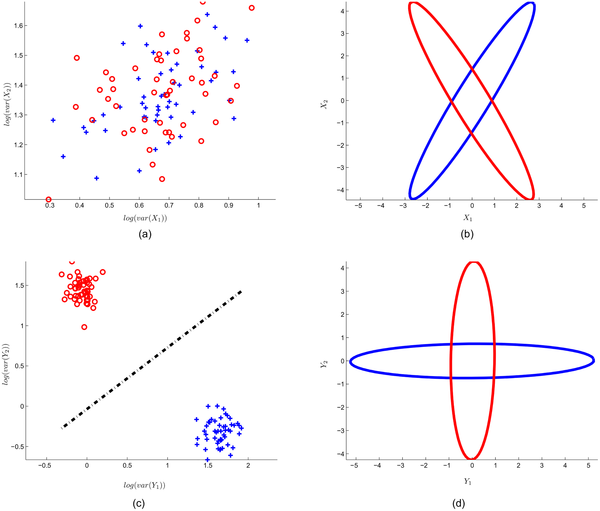
\includegraphics[width=12cm]{images/apple.png}
    \caption{林檎の図}
\end{figure}
  

\subsection{Common Spatiospectral Pattern(CSSSP)}
CSPではバンドパスフィルタ\(\cal H\)通過後の信号を扱ったため、バンドパスフィルタの設計を終えてからでなければCSPの問題を解くことができない。
しかし、バンドパスフィルタの設計次第ではCSPの解が変わることが想定される。そこで、バンドパスフィルタの設計をCSPの問題の中に取り込んだのがCSSSP\cite{csssp}である。

まず脳波信号\(X = \left[ x_1, \cdots, x_N \right] \in \mathbb{R}^{M \times N}\)に対して、
観測時間点を\(\tau\ > 0\)だけずらした\(X_{\tau} = \left[ x_{1+\tau}, \cdots, x_{N+\tau} \right] \in \mathbb{R}^{M \times N}\)を考える。
ここで$\tau = 1,\ldots,T$であり、$T$がFIRフィルタの次数の役割を担う。
更にクラス\( C_d \)に属する\( X \)に関して、
\begin{equation}
    \Sigma_{d}^{\tau} = \mathbb E_{X \in C_d} \left[ XX_{\tau}^T + X_{\tau}X^T \right]
\end{equation}
を定義する。ただし、\( \Sigma_{d}^{0} = \mathbb E_{X \in C_d} \left[XX^T \right] \)とする。FIRフィルタの実数係数ベクトルを$b=[1,b_2,\ldots,b_T]^T$として、
CSSSPの最適化問題は以下で表現される。
\begin{equation}
    \begin{aligned}
    & \max_{b_2,\ldots,b_T} \max_{w}
    & & w^T \left\{ \sum_{\tau = 0}^{T-1} \left( \sum_{j=1}^{T-\tau} b_j b_{j+\tau} \right) \Sigma_1^{\tau} \right\} w - \frac{\alpha}{T}|b|_1 \\
    & \text{subject to}
    & &  w^T \left[\sum_{\tau = 0}^{T-1} \left\{ \sum_{j=1}^{T-\tau}b_jb_{j+\tau} \right\} (\Sigma_1^{\tau} + \Sigma_2^{\tau}) \right] w = 1
    \end{aligned}
\end{equation}
この最適化問題では空間重みベクトル\(w \in \mathbb R^M\)とFIRフィルタの実数係数ベクトル$b$を同時に評価することが可能である。
目的関数における第二項は正則化項であり、$\alpha$はハイパーパラメータである。
この正則化によってFIRフィルタの系列ベクトルに対してスパース性が要請され、FIRフィルタが異常に複雑になることが避けられる。


\subsection{Filter Bank Common Spatial Pattern(FBCSP)}
CSSSPはFIRフィルタの設計をCSPの最適化問題に含むことで、バンドパスフィルタとCSPの同時最適化の定式化に成功した。
しかし、CSSSPによって求まる特徴量は1つのFIRフィルタを通過し、1つのCSPによって電極の重み付けが行われた脳波信号にすぎない。
クラス分類を行うことが最終目標であることを考えれば、この特徴量は必ずしも最適なものであるとは言い難い。
例えば左手の運動想起時と下肢の運動想起時では重要な周波数帯域が異なるためである。すなわちCSSSPによって決定されたFIRフィルタは、
左手の運動想起時に重要な周波数帯域を捉えている一方で、下肢に重要な帯域を失ってしまっているということが生じうる。FBCSPはこのような問題の解決を図る手法である。

まず、バンドパスフィルタバンク\(\{ {\cal H}_1, \ldots, {\cal H}_F \}\)を定義する。
各バンドパスフィルタを通過した\(\hat X_f = {\cal H}_f(X)\)に対して、それぞれCSPの問題を解くことで、複数の周波数帯域を反映した特徴量の抽出が可能となる。
しかし、この段階においてはCSSSPとは異なり、CSPとバンドパスフィルタの同時最適化を行ってはいないため、初めに定義したバンドパスフィルタバンクのCSP特徴量を対等に扱うことが妥当とは言えない。
FBCSPでは各バンドパスフィルタに対してのCSPの解から、
更に重要な特徴量の選定を行う方法までを含んだ提案がなされている\cite{fbcsp}。

\chapter{\mc 提案手法}
この章では初めに提案手法の大部分を占めるニューラルネットワークについて簡単に述べる。
その後、ニューラルネットワークを用いて運動想起型BCIを構築するアイデアと、
その具体的な提案モデルについて解説する。


%%%%%%%%%%%%%% 特徴量工学の説明 %%%%%%%%%%%%
\section{ニューラルネットワーク}

\subsection{フィードフォワードニューラルネットワーク}
特徴量工学はBCIに限らず、データ解析を必要とする多くの分野で活用されている。
例えば画像処理の分野では、画像に写っている物体の輪郭を
抽出するエッジ処理や、画像に対してぼかしを入れる平滑化処理などが特徴量抽出手法として用いられる。
また音声認識の分野では、音声の周波数に重要な情報が含まれていると考え、
周波数スペクトルやケプストラムなどを特徴量として用いる試みがなされてきた。

\subsection{リカレントニューラルネットワーク}

\subsection{畳み込みニューラルネットワーク}

\section{FIRフィルタと畳み込み層}
% \section{\mc スペクトログラムを画像とみなした手法(提案手法1)}
% \subsubsection{\mc 最大エントロピー法によるスペクトル密度推定}
% スペクトログラムの獲得には最大エントロピー法を用いる。
% フーリエ変換を用いたスペクトル密度推定法にはEEGには成り立たないであろう
% 仮定を要請しなければならないが、最大エントロピー法はウィーナー・ヒンチンの定理以外の一切の仮定を必要としないため、
% ロバストな推定が可能である。
% 最大エントロピー法のスペクトル密度推定法を時間窓をずらしながらEEGに適用することでスペクトログラムを獲得する。

% \subsubsection{\mc 画像認識の手法の適用}
% Convolution層は通常画像認識のために用いられるが、スペクトログラムからERDを検知する研究は従来より盛んであり、
% これは人間がERDを可視化、画像化してきたことに他ならない。
% スペクトログラムをERDの生じる周波数を特定するために用いるのではなく、
% 直接、畳み込みニューラルネットワークに与えることで分類させることを試みた。


\section{\rm FilterBank Network \mc(提案手法1)}
\subsubsection{\rm Convlution\mc 層によるFIR フィルタバンク}
EEGを\(X\in \mathbb R^{M\times N\times 1}\)とする。
ここに、\(M\)は電極の数、\(N\)はサンプル点数、\(1\)は後に周波数を示すためのダミーインデックスである。
\(X\)に対するConvolution層による演算は以下で表される。
\begin{equation}
    u_{m,n,k} = \sum_{c=1}^C\sum_{p=0}^{P-1}\sum_{q=0}^{Q-1} x_{m+p,n+q,c} h_{p,q,c,k} + b_{m,n,k}
\end{equation} 
この演算に関して、\(P=1,b_{m,n,k}=0,C=1\)でパラメータを与えることにより、
\begin{equation}
    u_{m,n,k} = \sum_{q=0}^{Q-1} x_{m,n+q,1} h_{1,q,1,k}
    \label{eq:pseudoFIR}
\end{equation} 
という演算を行うことができる。
ここでパラメータ\(H\in \mathbb R^{1\times D\times 1\times K}\)と与えることで、
フィルタ次数\(Q-1\)のFIRフィルタ\(K\)個からなるフィルタバンクとなる。

\subsubsection{\rm Convlution\mc 層による空間フィルタ}
続いて、第2層について\(Q=1\)でパラメータを与えることにより
\begin{equation}
    v_{m,n,l} = \sum_{p=0}^{P-1} u_{m+p,n,k} g_{1,q,1,k}
    \label{eq:pseudoFIR}
\end{equation} 
という演算を行うことが可能であり、EEGに対して電極の重み付けを行っていることに相当する。
ここで\(g\)がパラメータである。

以降ニューラルネットワークの演算を適宜定義することで、
2層目以降の層は、EEGを入力としたフィルタバンクからの出力を受け取ることが可能となる。
本研究では2層目以降もConvlution層のみを用いて特徴量の抽出を試みた。
提案手法におけるデータの形状の変化について図\ref{fig:pseudFBCSP}に示す。
\begin{figure}[t]
    \centering
    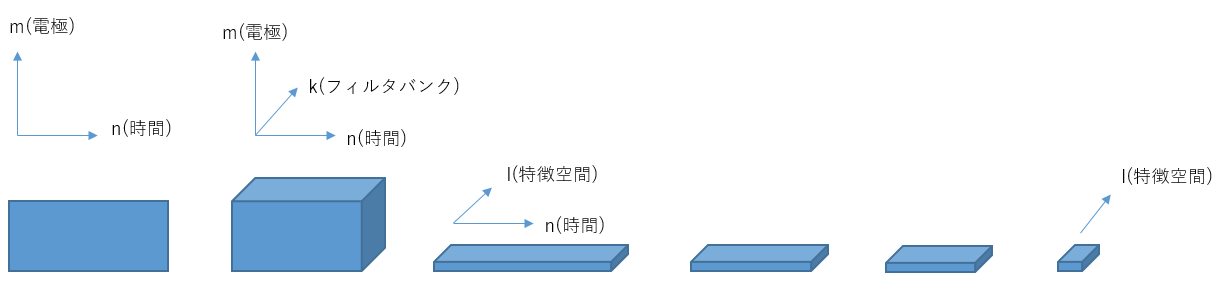
\includegraphics[width=13cm]{images/pseudFBCSP.png}
    \caption{Convlution層を用いたFIRフィルタバンクによるデータの形状変化}
    \label{fig:pseudFBCSP}
\end{figure}

同時に最適化可能な点である。具体的なニューラルネットワークの構造は実験結果と共に記す。


\section{\rm 3DConvlution + 2DConvLSTM\mc (提案手法2)}
\subsubsection{\mc 高階テンソルとしての \rm EEG\mc データ構造}
通常、EEGのデータは時間の次元を持つサンプル点数と空間的な情報を有する電極をインデックスとした
2階テンソルとして表現されるが、本論文では運動想起時のEEGは時間、電極、周波数をインデックスとした
高階テンソルで表されると仮定する。
この仮定はEEG従来より周波数帯域毎に異なる脳波として捉えられてきたこと、
特定の身体部位に対応する脳の領域が局所的であること、時系列データであることから妥当であると考えられる。

また電極のインデックスについては任意の配置によってテンソル化がなされるが、
頭皮上の空間的配置によって電極間の関連性は異なっている。
したがって時間、電極、周波数のインデックスに関して
電極のインデックスの取り方を2次元に展開し
時間、頭皮上の座標1、頭皮上の座標2、周波数をインデックスとする4階テンソルとして捉え直す。

この場合におけるEEGの測定データは
EEGが\(X\in \mathbb R^{M_1\times M_2\times N\times 1}\)と与えられ、
Convlution層を用いたFIRフィルタバンクは、3DConvlution層を用いることで以下の式で書き換えられる。
\begin{eqnarray}
    u_{m_1,m_2,n,k}& = &\sum_{c=1}^C\sum_{p_1=0}^{P_1-1}\sum_{p_2=0}^{P_2-1}\sum_{q=0}^{Q-1} x_{m_1+p_1,m_2+p_2,n+q,c} h_{p_1,p_2,q,c,k} + b_{m_1,m_2,n,k}\\
    u_{m_1,m_2,n,k}& = &\sum_{q=0}^{Q-1} x_{m_1,m_2,n+q,1} h_{1,1,q,1,k}
    \label{eq:pseudoFIR3D}
\end{eqnarray} 
\(u_{m_1,m_2,n,k}\)について\(m_1,m_2\)が頭皮上の座標を表すインデックスである。
3DConvlutionによるデータの形状の変化を図\ref{fig:pseudFBCSP3d}に示す。


\subsubsection{\rm ConvLSTM}
ConvLSTMは、通常のLSTMのLinear層の計算をConvolution層に変更することで
入力\(X = (X_1,\cdots,X_T)\in \mathbb R^{M_1 \times M_2 \times T \times K}\)を受け取り
出力\(Y = (Y_1,\cdots,Y_T)\in \mathbb R^{M_1' \times M_2' \times T \times C}\)を出力する。
ここに\(C\)は任意の正数であり、\(M_1',M_2'\)はパラメータの与え方で決定される。
この構造を入れることによって、
電極のインデックスを頭皮上に展開しフィルタバンクを通過した4階テンソルEEGを入力として受け取ることができる。
ここでConvLSTM内でのCovolution演算は頭皮上の2次元に対して行い、LSTMの処理は時間方向に行うようにする(図\ref{fig:ConvLSTM})。

この手法には頭皮空間上でEEGを観測しながら、
その時間経過を追うことで運動想起部位を分類するというモデルを構築する狙いがある。
また、頭皮上に展開された2次元に対してConvolution演算を用いることは、
電極配置が距離的に近い場合において強い関連性を有するという仮定が入る。
Convolutionの演算時にパラメータのサイズによって覆われる空間的領域以外の部分は
全く関連しないという無限に強い事前分布を与えることになるためである。
しかし実際にはConvolution層を積層することによって、空間的に離れた電極間にも
関連性を有する形に修正が可能であるため、事前分布を与えながらも、
実際の関連性の探索はニューラルネットワークの学習によって獲得される。
\begin{figure}[t]
    \centering
    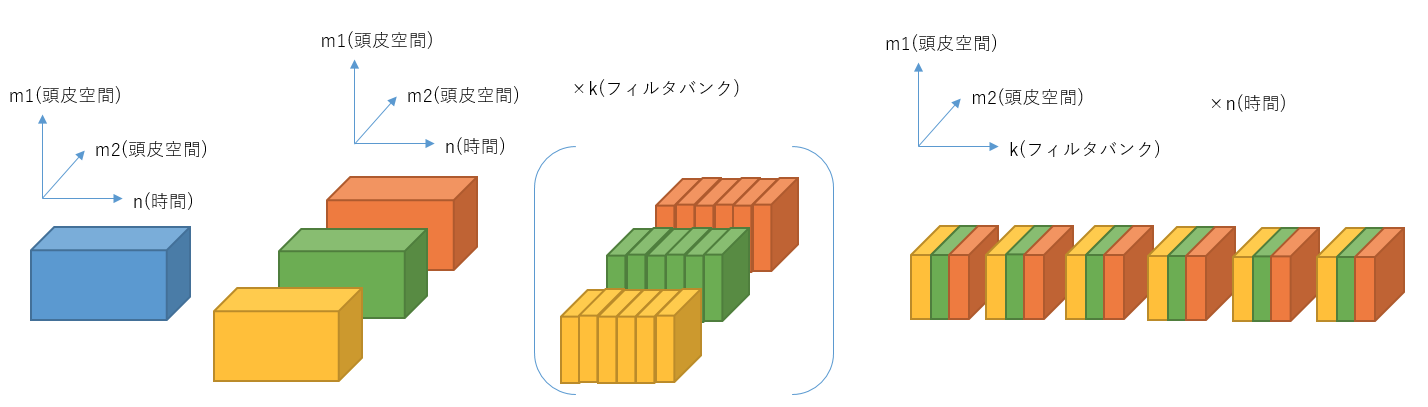
\includegraphics[width=13cm]{images/pseudFBCSP3d.png}
    \caption{3DConvlution層を用いたFIRフィルタバンクによるデータの形状変化}
    \label{fig:pseudFBCSP3d}
\end{figure}
\begin{figure}[t]
    \centering
    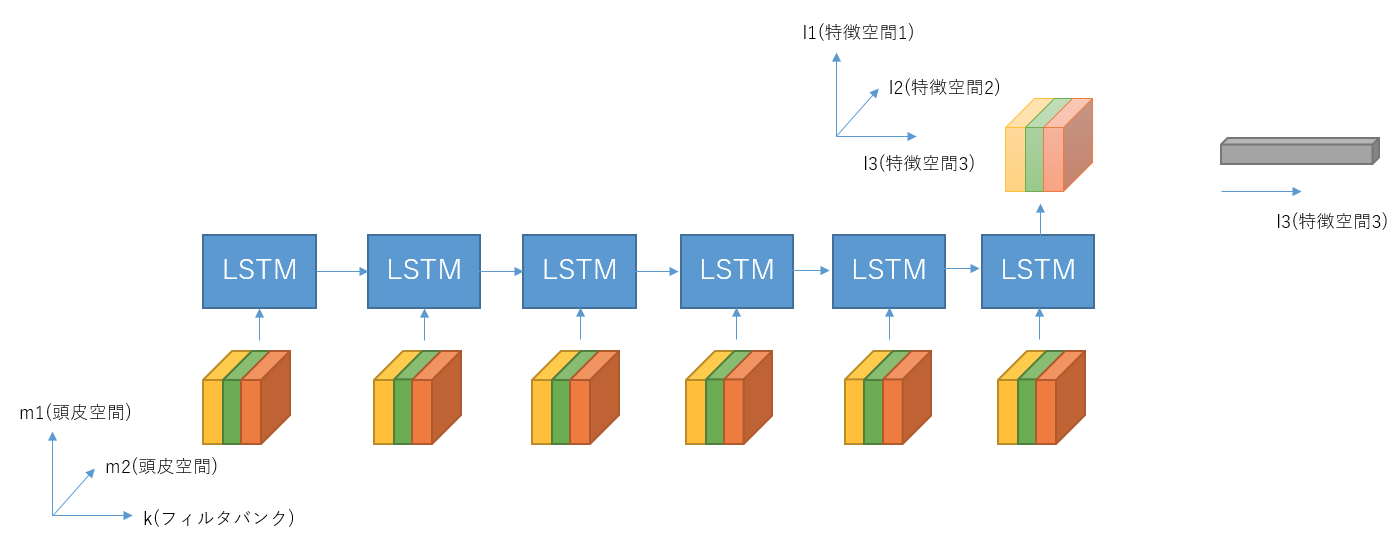
\includegraphics[width=13cm]{images/ConvLSTM2d.png}
    \caption{ConvLSTMによるデータ形状変化}
    \label{fig:ConvLSTM}
\end{figure}

このような仮定を置くことの妥当性を示すものとして、
信号源推定を行う際にグラフフーリエ領域へ変換を行うことで
良い推定結果が得られるという東らの研究\cite{グラフフーリエ}がある。
グラフフーリエでも、空間的に距離の近い電極によって測定されるEEGほど
類似性が高いという仮定が決定論的に与えられる。

\input{chapter/chapter4/3DpseudoFBCSP}
\input{chapter/chapter4/3Dconv_and_2DconvLSTM}
% \section{\mc 従来手法のまとめ}
運動想起型BCIは、様々な特徴量抽出手法と分類手法を適宜組み合わせて構築されている。
数多くの手法が以下に示す脳波に関する知見を意識している。
\begin{itemize}
    \item 運動想起する身体部位に応じて、強く反応する頭皮領域は異なる。
    \item 事象関連脱同期は、特定の周波数領域に生ずる。
    \item 個人差や計測環境の影響を受けやすい。
\end{itemize}
空間フィルタや
バンドパスフィルタあるいは時間周波数解析を用いること、
また複数の分類手法を比較しなければならないことの理由が
上記の脳波の性質に集約されている。
このセクションでは、多数存在する運動想起型BCIの構築方法に関して、
統一的な視点に立って概観する。その後、従来手法全般に対する問題点を提示し、このチャプターを終える。

\subsection{\mc 特徴量の観点からの従来手法}
運動想起を1回行った際に計測された脳波を以下で表記する。
\begin{equation}
    X =(x_1, \cdots, x_N)\in \mathbb{R}^{M \times N}\    
\end{equation}
ここに\(M\)は電極の個数、\(N\)は計測時間点数である。
空間フィルタは\(W\in \mathbb R^{M \times M}\)によって
脳波を\(W^TX \in \mathbb R^{M \times N}\)と変換する。
通常は更に電極の軸に関して次元削減を行うが、ここでは単に線形変換とする(必要であれば、後に削除すれば良い)。
時間周波数解析\(h(\cdot)\)は時間的に局在する基底関数を\(K\)個準備した場合、
各時間\(n\)において信号を基底関数の重ね合わせで表現した際の係数\(h(X) \in \mathbb R^{M \times N \times K}\)へと変換する。
空間フィルタと時間周波数解析の両方を用いる場合には、以下の形式で表される特徴量を抽出する。
\begin{equation}
    Z = h(W^TX) \in \mathbb R^{M\times N \times K}
    \label{eq:EEGfeatures}
\end{equation} 
一方でフィルタバンクを用いるFBCSPなどは以下の形式で表すことができる。
\begin{eqnarray}
    && {\cal H}  =  \{ {\cal H}_1,\cdots, {\cal H}_K \} \\
    && \hat X_k  = {\cal H}_k(X) \in \mathbb R^{M\times N} \\
    && Z_k  = W_k^T{\cal H}_k(\hat X_k) \in \mathbb R^{M\times N} \\
    && Z  =  (Z_1,\cdots, Z_K) \in \mathbb R^{M\times N \times K}
    \label{eq:EEGfeaturesbandpass}
\end{eqnarray} 
ここに\({\cal H}\)はフィルタバンクであり、\(K\)はフィルタの個数に相当する。
いずれにしても、抽出される特徴量は\(Z\in \mathbb R^{M\times N \times K}\)という
3階テンソル(電極×時間×周波数)である。

A. S. Aghaei\cite{Ztfc}も同様のことに言及しており、脳波\(X\)から\(Z\in \mathbb R^{M\times N \times K}\)
を獲得する様々な手法について比較している。
更に\(Z\)が得られた後の次元削減および運動想起部位を出力する分類器も含め、
一連の手法に関して、
電極軸と周波数軸に対する双線形変換によるアプローチを提案している(図\ref{fig:fbcsp bilinear}(b,c))。
図中で``space"と表現されている単語は本論文中では電極に相当する。\(\Omega\)は運動想起部位であり、
\(\hat \Omega\)がBCIの予測出力である。
\begin{figure}
    \centering
    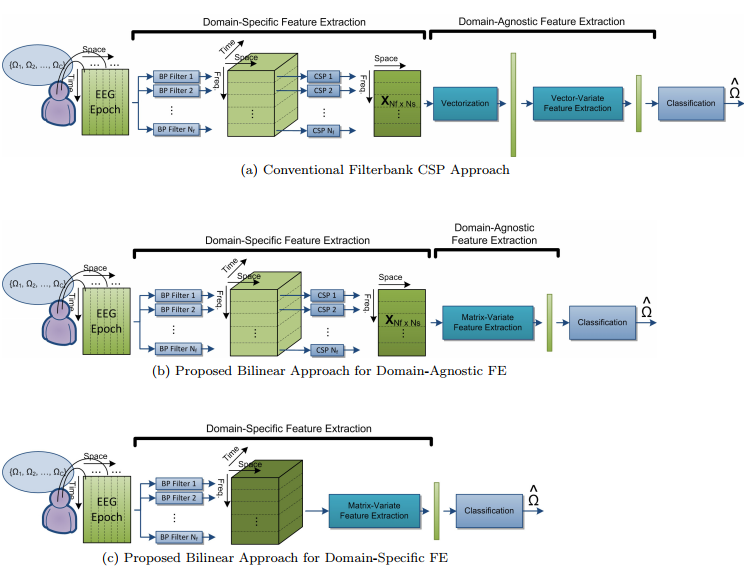
\includegraphics[width=14cm]{images/bilinear.png}
    \caption{脳波を3階テンソルとした手法の模式図(参照\cite{Ztfc})}
    \label{fig:fbcsp bilinear}
\end{figure}


\subsection{\mc 構成の観点からの従来手法}
次に典型的な運動想起型BCIの構成について述べる。
典型的な運動想起BCIは、運動想起に関連している脳波を取り出すための前処理\(\cal H(\cdot)\)
によって脳波の生データから\(\hat X\)を獲得することが一般的である。
\begin{equation}
    \hat X = {\cal H}(X)
    \label{eq:bandpass}
\end{equation}
次に、運動想起に関連している電極を選定するための空間フィルタ\(f(\cdot)\)を適用する。
\begin{equation}
    Z = f(\hat X)
    \label{eq:spatfilter}
\end{equation}
続いて\(Z\)に対して、
運動想起部位\(Y\)を出力する分類器\(g(\cdot)\)を準備することで、運動想起BCIが構成されている。
\begin{equation}
    Y = g(Z)
    \label{eq:classifier}
\end{equation}
従って、BCIは脳波\(X\)を引数とした合成関数という形式を取る。
\begin{equation}
    Y = (g\circ f \circ {\cal H})(X)
    \label{eq:bci_gosei}
\end{equation}
典型的なCSPを用いたBCIでは\(\cal H\)をバンドパスフィルタ、\(f\)をCSP、\(g\)をLDAやSVMによって個別に構成する。
ここで\(f^*(\cdot)=(f\circ{\cal H})(\cdot)\)として、バンドパスフィルタとCSPを同時に構成することを考えればCSSSPによるBCIになり、
\(\cal H\)をフィルタバンクにすることでFBCSPによるBCIとなる。
一方で時間周波数解析に基づくBCIでは変換(\ref{eq:time-freq})を\(h(\cdot)\)として、
\begin{equation}
    Y = (g\circ h \circ f \circ {\cal H})(X)
    \label{eq:bci_gosei2}
\end{equation}
という形式で表せる。この時、\(\cal H\)や\(f\)はERDを検出するための
神経科学的な知見に基づいた設計がなされる場合もあれば、機械学習の手法が用いられる場合もある。
更に時間周波数解析によって得られるパワースペクトログラムに対して
非負値行列分解などを用いて特徴量を抽出する試みもある\cite{kNMF,kNMF2}。
この場合も行列分解による変換を\(a(\cdot)\)と置けば
\begin{equation}
    Y = (g\circ a\circ h\circ f\circ {\cal H})(X)
    \label{eq:bci_gosei3}
\end{equation}
と表され、形式上は合成関数である。それぞれの関数の役割を明示しなければ、BCIは単に以下の合成関数である。
\begin{equation}
    Y = (f_K\circ \cdots \circ f_1)(X)
    \label{eq:bci_gosei4}
\end{equation}
BCIを合成関数(\ref{eq:bci_gosei4})を出発点にして見ると、
従来のBCI構築手法は、合成関数に含まれる関数の数を明確にし、
それぞれに役割を付与し、与えた役割を担うような調整が個々に行われていると見なせる。
ただし、関数\(f_i\)を設計するためには\(f_{i-1}\)の設計が終了していなければならない。

% 個々の関数\(f_i(\cdot)\)を設計する場合には、その候補となる関数族\(\{f_i(\cdot,\theta_i)\mid \theta_i \in \Theta_i\}\)を仮定する。
% ここに\(\Theta_i\)は\(\theta_i\)が取りうる全ての値の集合である。
% 例えば、CSPを用いた\(Y = (g_{lda}\circ f_{csp} \circ {{\cal H}_{buttord}})(X)\)で表されるBCIを考え、
% バタワースバンドパスフィルタ、CSP、LDAについて設計を行う場合は以下の関数族を仮定する。
% \begin{eqnarray}
%     {\cal H}_{buttord}(\cdot) &=& \{{\cal H}(\cdot,w_p,w_s,r_p,r_s) \mid w_p,w_s \in \mathbb R^2, r_p,r_s \in \mathbb R\} \\
%     \label{eq:H_buttord}
%     f_{csp}(\cdot) &=& \{f(\cdot, W_{csp})\ \mid W_{csp} \in \mathbb R^{m\times M} \}\\
%     \label{eq:f_csp}
%     g_{lda}(\cdot) &=& \{g(\cdot,W_{lda})\ \mid W_{lda} \in \mathbb R^{d \times m}\}    
%     \label{eq:g_lda}
% \end{eqnarray}
% \(w_p,w_s\)はそれぞれ通過帯域コーナー周波数、阻止帯域コーナー周波数である。
% \(r_p,r_s\)はそれぞれ通過帯域リップル、阻止帯域の減衰量である。
% \(W_{csp}\)はCSPにおける線形変換の表現行列であり、
% 電極数\(M\)の次元を持つ脳波を\(m (< M)\)の任意の次元の電極空間に圧縮する。
% \(W_{lda}\)はLDAにおける線形変換の表現行列であり、
% \(m\)次元の電極空間から分類クラスの数より小さな任意の\(d\)次元への射影を担う。
% ここではバンドパスフィルタのパラメータに関しては人手で決定され、
% CSPとLDAのパラメータはそれぞれの学習アルゴリズムによって決定される場合を想定する。
% ここで例に挙げたBCIは\({\cal H}_{buttord}\)の設計を終えなければ、\(f_{csp}\)の設計に入ることはできない。
% あるいは結果が期待通りでなかった場合には、\({\cal H}_{buttord}\)の設計に戻らなければならない。
% \({\cal H}_{buttord}\)が\(f_{csp}\)の学習結果にどのような影響を及ぼすのかは定かではないため、
% この後戻り設計は試行錯誤によって解決するしか無い。
% 一方でCSSSPはこの問題を解決した手法であると言えるが、
% 同様の問題が\(f_{lda}\)と\(f_{csp}\)の間にも存在する。





\chapter{\mc 実験方法}
この章では実験に用いたデータについて説明し、
その後、データを用いた実験に対してどのような評価を行うのかを明示する。

\chapter{\mc 結果と考察}
この章では従来手法と提案手法の実験結果をそれぞれ示す。
結果に対して考察と本研究の結論を述べ、更に今後考えうる改善案などについて簡単に述べる。

%
%
\appendix
%
\renewcommand{\thechapter}{A}
\stepcounter{chapter}
\def\theequation{A.\arabic{section}.\arabic{equation}}
\makeatletter
\@addtoreset{equation}{section}
\makeatother
\chapter*{Appendix}
\addcontentsline{toc}{chapter}{Appendix}


\section{$B%;%/%7%g%s(B}

\subsection{$B%5%V%;%/%7%g%s(B}




%
%
\chapter*{謝辞}
% \addcontentsline{toc}{chapter}{謝辞}
...
...


% \begin{thebibliography}{99}
%     \bibitem{csssp} Guido Dornhege, Benjamin Blankertz, Matthias Krauledat, Florian Losch, Gabriel Curio, Klaus-Robert M?ller,
%         ``Combined optimization of spatial and temporal
%         filters for improving Brain-Computer Interfacing
%         '',
%         {\it IEEE TRANSACTIONS ON BIOMEDICAL ENGINEERING},
%         Vol. XX,
%         No. Y,
%         2006.

%     \bibitem{fbcsp} Kai Keng Ang, Zheng Yang Chin, Haihong Zhang, Cuntai Guan
%         ``Filter Bank Common Spatial Pattern (FBCSP) in Brain-Computer Interface'',
%         {\it IEEE TRANSACTIONS ON BIOMEDICAL ENGINEERING},
%         {\it in Proc. 2008 Int. Joint Conf. Neural Netw.},
%         pp. 2390-2397,
%         2008.

%     \bibitem{deepconv} Robin Tibor Schirrmeister,
%         Jost Tobias Springenberg,
%         Lukas Dominique Josef Fiederer,
%         Martin Glasstetter,
%         Katharina Eggensperger,
%         Michael Tangermann,
%         Frank Hutter,
%         Wolfram Burgard,
%         ``Deep learning with convolutional neural networks for EEG decoding and visualization'',
%         {\it Human Brain Mapping},
%         Vol. 38,
%         No. 11,
%         pp. 5391-5420,
%         2017.
%     \bibitem{csp_eigen} B. Blankertz, M. Kawanabe, R. Tomioka, F. Hohlefeld, V. Nikulin, 
%         and K. R. M¨uller, “Invariant common spatial patterns: Alleviating
%         nonstationarities in brain-computer interfacing,” {\it Advances in
%         Neural Information Processing Systems}, vol. 20, pp. 113-120, 2008.
%     \bibitem{cvscsp} Jyoti Singh Kirara, R. K. Agrawala, 
%         ``Optimal Spatio-Spectral Variable Size Subbands Filter For Motor
%         Imagery Brain Computer Interface'',
%         {\it  Procedia Computer Science },
%         84, 14-21, 2016.
%     \bibitem{ICA1}
%         Hiromu Gotanda, Takaaki Ishibashi, Nobuo Iwasaki, Katsuhiro Inoue,
%         ``独立成分分析の基礎と応用'',
%         {\it 数理解析研究所講究録},
%         第 1743 巻, 6-20, 2011.
%     \bibitem{ICA2} Noboru Murata, ``入門独立成分分析'', 東京電機大学出版, 2004.

% \end{thebibliography}
%
\bibliography{reference}
% \bibliographystyle{jplain}
\bibliographystyle{junsrt}

%
% \include{reference_acknowledgment}
%
%
\newpage
\printindex
%
%
\end{document}
